\part{Case Studies} % Main chapter title

\label{part:case_studies} % Change X to a consecutive number; for referencing this chapter elsewhere, use \ref{ChapterX}

\lhead{Part 1. \emph{Case Studies}} % Change X to a consecutive number; this is for the header on each page - perhaps a


In any application that is not entirely composed by repetitive, precomputed actions, robots need reasoning skills, which severely depend on the quality of the representation of the current environment. This representation can be more or less complex, depending on the application. 

Imagine, for example, a robot whose task is cleaning the floor of a room. In the simplest case, this robot would only be provided with an elementary set of sensors. Without the capacity to understand which areas actually need cleaning, this robot could only move through the room, randomly or with some strategy, achieving the task in a longer amount of time than what would actually be needed. 

% In a fairly simple case, this robot would rely on a map of the room and a set of lasers, or bumper sensors, to detect obstacles. 

Now, imagine a household robot that needs to actively help a family that lives in an apartment, by fetching objects, providing information, and helping to accomplish various tasks. Let us imagine that one of the members of the family, Greg, is moving in the living room, searching around, while exclaming `Where are my glasses?'. In the ideal situation, our robot would try to help Greg, by giving him information such as `They are on the table to your right', or even by fetching them for him. 

Clearly, in this scenario, the robot needs deeper reasoning skills. It needs to understand that the user is looking for its glasses, to link them to their actual physical location, to compute the spatial relationship between the table and the glasses, and to provide information in a natural way. In fact, if the robot would tell Greg that the glasses are in the position $(3.2, 5.0 , 1.3)$, Greg would very likely be very perplexed. A more natural way would be to inform Greg that his glasses are on a table, whose location is pointed taking into account Greg's position.

In this case, having sophisticated sensors is, of course, important but not sufficient. The robot needs also to \textit{reason} on the sensor's data in order to produce meaningful information. For example: laser points and camera images need to be integrated to recognize objects and humans; spatial relationships  (e.g. the glasses are on the table) have to be properly modeled; actions performed by humans, and their effects on the environment, need to be recognized; and so on. 

The process of reasoning on data to produce symbolic information is called \textit{situation assessment}. Endsley explained in \cite{endsley1995toward} that this process is deeply linked to the quality of  decions of the robot.

While in many applications robots can benefit from a situation assessment component, being able to perform complex reasoning on data is particularly important in HRI. If the robot is able to take better decisions (i.e.  efficient, safe, socially acceptable, natural) than it will be perceived in a more positive manner by humans. 




                 % Chapter Template

\chapter{Situation Assessment} % Main chapter title

\label{chap-situation_assessment} % Change X to a consecutive number; for referencing this chapter elsewhere, use \ref{ChapterX}

\lhead{Chapter . \emph{Situation Assessment}} % Change X to a consecutive number; this is for the header on each page - perhaps a shortened title

In this chapter we introduce the Situation Assessment capacities of our system. 

%TODO: Citations on Toaster. Look and add other possible citations. Cite everything. Everything!
\section{Introduction}
\label{sec:situation_assessment-intro}
\subsection{What is Situation Assessment?}
%Motivation
In any application that is not entirely composed by repetitive, precomputed, actions, robots need to possess adeguate reasoning skills, which severely depend on the quality of the representation of their environment. This representation can be more or less complex, depending on the application. Imagine, for example, a robot that needs to clean the floor of a room. For a fairly simple case, this robot would rely on a map of the room and set of lasers, or bumper sensors, to detect and obstacles. Now, imagine a household robot that needs to actively help a family that lives in an apartment, by fetching objects, providing information, and helping accomplish various tasks. Clearly, in this situation, the robot needs a deeper degree of reasoning on sensor data: laser points and camera images need to be integrated to recognize objects and humans; spatial relationships  (e.g. the cup is on the table, the human has the cup) need to be properly modeled; actions performed by humans, and their effects on the environment, need to be recognized; and so on. 

In this situation, there is a need for a process which performs different kinds of reasoning on perceptual data, and produces information that can be used by the rest of the system. This process is called situation assessment, and is deeply linked to the quality of the decisions of the robot, as explained by Endsley in \cite{endsley1995toward}. 


%what are people doing with situation assessment and belief management
Situation assessment components have been designed by different authors, but they are usually developed for specifc applications, like in \cite{Chella2010,Kluge01situationassessment}. In \cite{beetz2015robosherlock}, instead, the authors present ROBOSHERLOCK, an opersource framework that can be used to implement perception systems. Among its features, ROBOSHERLOCK supports logical queries about the world state, and so supporting task-driven situation assessment. 

\subsection{Theory of Mind}
An important part of Situation Assessment is representing other agents in the environment, not as simple obstacles, but as acting entities, with different beliefs on the state of the world, and with the capacity to affect the environment. 

Theory of Mind \cite{premack1978does} is a skill used to reason about humans' beliefs and thoughts, and how they affect actions. An ability linked to this concept is perspective taking, which is widely studied in developmental literature.  Flavell in \cite{flavell1977development} describes two levels of perspective taking: 
1) perceptual perspective taking,  the capacity to understand that other people see the world differently ~\cite{Tversky1999}; and 2) conceptual perspective taking, the capacity to attribute thoughts and feelings to other people ~\cite{Baron1985}. Studies on individuals that don't possess the required mechanisms to perform perspective taking, like young children \cite{frick2014picturing}, have put into light the difficulties these people have to accomplish everyday social relationships and confirmed the importance of this ability.

Previous works in robotics have shown that enhancing the robot's perspective taking abilities improves its reasoning capabilities, leading to more appropriate and efficient task planning and interaction strategies \cite{Trafton2005,ros2010one}. \cite{breazeal2006} showed that perspective taking can even enhance learning by imitation processes, allowing the viewer to learn a task from "flawed" demonstration, which may be correct from the teacher's point of view but are actually ambiguous. 

An important study linked to conceptual perspective taking is the 'divergent belief task'.  Formulated in~\cite{wimmer1983}, this kind of task requires the ability to recognize that others can have beliefs about the world that differ from the observable reality. ~\cite{BreazealGB09} proposed one of the first human-robot implementations, resulting in more advanced goal recognition skills. 

Not many frameworks throughly model different agent's beliefs.  Scheutz \cite{scheutz2013computational}) studied this problem, developing a computation model to represent agent's mental states. The work is oriented in particular toward communication problems and not geometrical and spatial perspective taking issues.

\subsection{Intention Recognition}
%TODO: here in particular we need something for action recognition
Another crucial skill of a robot that interacts with human is recognizing others' actions and goals. Recognizing others' goals is directly linked to modeling humans' beliefs, since, as explained by \cite{byom2013theory} "as humans, we generally believe that others act in ways that are consistent with their beliefs and goals". In psychology \cite{bruner1981} and philosophy \cite{bratman1984} literature, an intention as the wish and will to achieve a goal. Intentions memerge from contextual causes (motivations) and are present the goal is achieved or abandoned, pushing agents to undertake actions leading to that goal.

The recognition of human activities is an important topic in computer science research, which can be studied at different levels. Anticipating human actions and movements allows the robot to adapt its behavior and proactively help humans, as studied in \cite{koppula2013anticipating}. An interesting idea is using the robot's own internal models in order to recognize actions and predict user intents, as shown by the \textit{HAMMER} system in \cite{demiris2007prediction}. Sequences of actions can be linked to plans, a well-known topic called plan recognition. Several approaches have been studied in this domain using, for example, classical planning \cite{ramirez2009plan}, probabilistic \cite{bui2003general} or logic techniques \cite{singla2011abductive}.  In \cite{talamadupula2014coordination}, the authors use classical planning, with an efficient replanning strategy, in order to infer user's intentions. The system has been implemented on a PR2 robot and tested on a collaborative scenario. \cite{breazeal2009embodied} presents an architecture in which the robot is able to use its own schemas and models to infer human actions and goals, and to proactively help him achieve them. Shared plans are not explicitly represented in the system, and the robot helps the human by mapping the inferred goal information in its own beliefs, and choosing appropriate action

Two approaches that can be used for intention estimation are Interactive Partially Observed Markov Decision Processes (I-POMDP) and Inverse Learning. I-POMDP  \cite{gmytrasiewicz2004interactive} offer a rich framework that extends Partially Observed Markov Decision Processes (POMDP) in a multi-agent setting. Inference in these models can be extremely complex, but there have been attempts at solving this issue, like in \cite{doshi2009monte,hoang2013interactive}. 

Inverse Reinforcement Learning \cite{ng2000algorithms} formulates the problem of computing an unknown reward function of an agent after observing his behavior. This strategy has been applied, with Bayesian Networks (BN), in \cite{Nagai2015}, in order to learn the mental model of another agent, and choose appropriate actions for a relationship building task. A linked approach is inverted planning, which has been applied in a bayesian framework in \cite{baker2009action}  for human action understanding.

Contextual information can be used to further disambiguate complex situations. \cite{Liu2014} shows a system using BNs to understand users' intentions with an emphasis on contextual information.

It is very important to consider humans' beliefs when estimating their intentions. In a dynamic environment, agents can execute actions, modifying the state of the world without other agents being able to perceive the changes. Let us imagine a scenario. Bob comes back home from work and would like to relax while reading. He lays down on a sofa with a book, and reaches to a nearby table to grab his glasses. He does not know that his wife, during the day, moved the glasses to another room. If we would ignore Bob's beliefs on the world (i.e. he does not know that the glasses are not on the table) we could infer that, for example, Bob would like a drink while he is sitting on the sofa, or the tv remote controller. If, instead, we would know that Bob thinks his glasses are on the table (and we would use other contextual information perhaps, like Bob's habitudes) we would be able to correctly infer Bob's current intention, that is, taking his glasses, and warn him that they are not there, perhaps even fetching them for him. In robotics, an interesting framework that considers this issue is the Bayesian Theory of Mind \cite{baker2014modeling}, used to represent the inference process of an observer looking at another agent's behaviors, with POMDPs and Dynamic Bayesian Networks (DBNs).


\subsection{Dialogue}
Dialogue is a very important part of situation assessment. Agents often communicate, while executing a task together, or even when working independently, to clarify ambiguities and obtain missing information. While we will not present a specific dialogue component in this work, we have used our system in \cite{Ferreira2015}, where our belief management component and a situated dialogue system were implemented in a simulator. This model was compared with a basic system (without belief awareness) in a study with 60 interactions, in a simulated environment. We successfully showed that the dialogue management system significantly improves its efficiency, reducing the number of dialogue turns in the interaction, and its accuracy, with a higher success rate when a divergent belief situation appears.

\section{System Overview}
\label{sec:situation_assessment-overview}

In our architecture, we built a Situation Assessment layer, which is able to:
\begin{itemize}
\item  Detect and track entities.
\item  Process sensor data in order to produce symbolic information.
\item  Maintain a belief model for each agent.
\item  Infer human actions and intentions. Our system is able to perform this estimation by taking into account the current belief of humans on the world state. 
\end{itemize} 

This layer is composed by different elements, as shown in Fig. \ref{fig:situation_assessment-situation_assessment_overview}.
\begin{itemize}
\item Sensor Data. Data produced by different possible sensors (e.g. lasers, camera, etc.)
\item Entity Detection. Different components detect and track humans and objects in the environment.
\item Human Inputs. Users can communicate with the robot by using a tablet application.
\item Human Interface. User inputs from the tablet are elaborated into commands, to introduced in the Database.
\item Geometrical Reasoning. Symbolic facts are produced starting from perceptual data.
\item Belief Management. The system maintains a mental model of each agent.
\item Intention and Action Recognition. Human actions and intentions are inferred based information provided by the Geometrical Reasoning and on the belief models of the agents.
\item Database. The database stores symbolic facts produced by the system.
\end{itemize}


 \begin{figure}[h!]
	\centering
	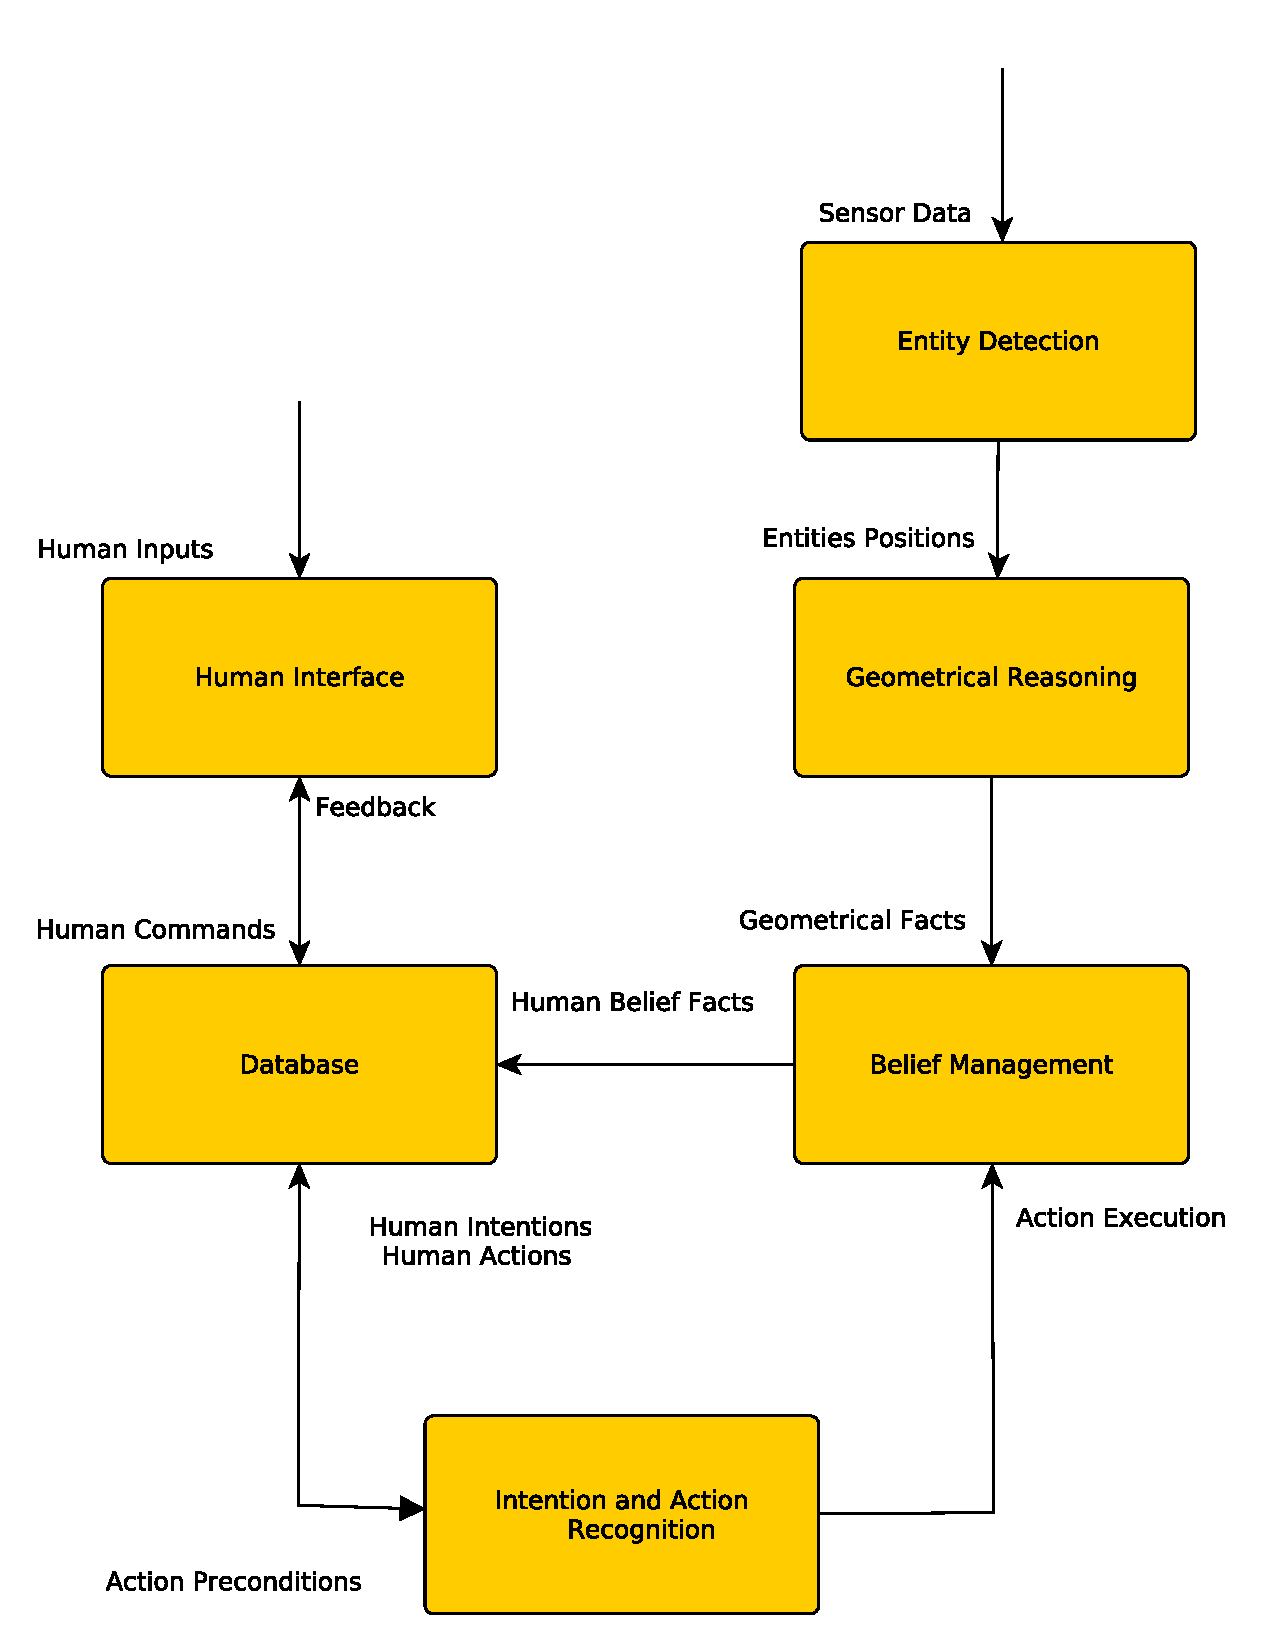
\includegraphics[scale=0.45]{img/situation_assessment/situation_assessment_overview}
	\caption{Overview of the different modules composing the Situation Assessment Layer}
	\label{fig:situation_assessment-situation_assessment_overview}
\end{figure}


In addition, the system possesses a description of the world, with a definition of all the elements known to the robot, like objects and agents, possible actions, possible intentions, intentions, etc. 
Symbolic facts are constantly produced starting from the sensor data and from the position of entities, and then the Belief Manager will update and maintain the belief model of each agent. The belief model of humans and of the robot will be used by the Intention and Action Recognition modules to infer the most likely intentions and actions performed. All these information are introduced in the Database, and can be read by other components. For example, the Goal Manager can choose a goal based on human commands or on an estimation of its intention. In a similar way, the Action Execution modules will read the Database in order to obtain the state of the world, to check action preconditions.  

Our situation assessment layer was presented in \cite{Milliez2014}, where it was used to pass the Sally and Anne test~\cite{Baron1985} on a robotic platform. The intention and action recognition capacity was introduced in \cite{devin2016some}.

\section{Object and Human Detection}
In our system, we chose to simplify perception issues, focusing on reasoning aspects. We associate a unique tag to every object that is interesting in a particular scenario.  When the robot observes a tag using a camera, it detects the corresponding object using a tag-matching algorithm.
Regarding humans, we use a motion capture software to identify and track agents moving in the environment. Using different tags, we can track the head, shoulders, and right arm of a human. Our situation assessment component has also been tested using a laser and RGB based detector in the SPENCER european project \footnote{http://www.spencer.eu/}.

\section{Human-Robot Communication}
Similarly, communication between the human and the robot is limited, in our system. Humans can give commands to the robot by using a tablet application, where they can manage the robot goals, by adding a new goal, canceling a previous one, or pausing the robot. The robot is able to provide simple verbal output by using a text-to-speech component. The robot is not able to perform real dialogues with the human but it can adapt its speech to the current tasks and scenarios, by explaining plans, informing the human if it has a problem, verbalizing its current actions, and so on. This feature will be explained fully in chapter \ref{chap-plan production and management}. 

\section{World Model and Geometrical Reasoning}
\label{sec:situation_assessment-situation_assessment}
The first step in estimating human intentions is reasoning about the environment and the belief of humans. Our world is composed by agents, the robot and humans; by objects; and by areas, which are bounded regions in the environment with semantic meaning, e.g. living room, kitchen. To be more generic, we will sometimes use the word \textit{entity} to refer to an agent, an agent's joint or an object. We can assign properties, to entities and areas to represent different information, e.g. 
an agent can be in a specific area, a box can be opened and can contain objects, a bottle can contain liquids, a mug can be hot. The $subject$ of a property is the name of the primary entity linked to it (e.g. bob, mug). 
 We divide properties in two classes: 
\begin{itemize}
\item fully observable:  can be seen by any present agent looking at the linked entity or area, e.g. the box is open
\item partially observable: can be observed by present agents only in specific situations, represented as rules linked to the object and the property, e.g. an agent can see that a box contains items only when it is open, an agent can detect that the mug is hot only when he touches it.
\end{itemize}

Using its perception abilities the robot can build a representation of the environment, starting with entities' positions. Using geometrical reasoning we can compute spatial relationships between entities, e.g. the glasses are on the shelf, the human is moving toward the library, the glasses are reachable by the human, the bottle is visible for the human. These reasonings provide a base for the perspective taking abilities of the robot. 


\section{Belief Management}
\label{sec:situation_assessment-belief_management}
In our system, agents can have divergent representations of the world. To model this aspect, the information produced by perception, geometrical reasoning and inference, are collected by the robot in \textit{belief models}, built for itself and for each agent. A \textit{belief model} is a symbolic representation of the world state, as known by an agent. In a model, the world state is represented by properties and values. To represent the lack of knowledge of an agent, the value of a property can be \textit{unknown}.

We consider our world as a dynamic environment, where properties can change and actions can be performed.  We define an action as a tuple $(name, preconditions, target, postconditions)$. The $name$ of an action is a unique string that identifies it. The $preconditions$ are a list of properties that must be true in order to realize the action. In our system, an action is executed on a $target$, which can be a physical object, like a cup, but also an area of the environment, like a room. The $postconditions$ are the set of properties, and their values, affected by the action's execution.

Since we are interested on reasoning and not perceptual aspects, we use inference, as explained in Sec. \ref{sec:situation_assessment-intention_recognition}, in order to understand when a human has performed an action. Through the predefined $postconditions$ of actions we can also infer changes in object properties, e.g. the human opens a box, so the box is now open. 

We created a rule based framework in order to build the beliefs of each agent and update them when needed. Human belief models are updated using the perspective taking skills of the robot. When the robot detects the execution of an action in the world, it updates the belief model for itself and for every human that can perceive the action, adding the action's $postconditions$ to their models. When an action is not perceived by a human (e.g. the user was in an other room), his belief model will not be updated, as he is not aware of the changes that occurred.

However, when he comes back and looks at the environment, we assign him a new belief state following a set of rules, which we will now explain. We call $H$ the agent, $HB$ his belief model, and $RB$ the robot's belief model. We also create the following predicates: $obs(p)$ means that the instance of property $p$ is observable, $valid(p,x)$ means that the instance of property $p$ doesn't contradict the current perception data of agent $x$, $value(p,m)$ is the value of predicate $p$ in belief model $m$, and $vis(p,x)$ means that agent $x$ has visibility on the linked entities of property $p$. The rules for the $valid$ predicate will be different in each property. For example the property \textit{MUG isOn TABLE} won't be valid for agent Max if he can see that there is no mug on the table. For each property $p\in HB \cup RB$:
\begin{itemize}
\item if $p \in RB, \quad p\not\in HB,\quad obs(p),\quad vis(p,H) \rightarrow value(p,HB)=value(p,RB)$.
\item if $p \not \in RB,\quad p\in HB,\quad obs(p),\quad vis(p,H) \rightarrow remove\quad $p$ \quad from \quad HB$.
\item if $p\in RB,\quad p\in HB$ then:
	\begin{itemize}
      \item if $value(p,HB)\neq value(p,RB),\\ \quad obs(p),\quad vis(p,H) \rightarrow \\ value(p,HB)=value(p,RB)$.
      \item if $value(p,HB)\neq value(p,RB),\\ \quad !obs(p),\quad !valid(p,H) \rightarrow \\ value(p,HB)=\textit{unknown}$.
	\end{itemize}
\end{itemize}
The idea of this set of rules is updating an agent's mental belief model for a property only if it's observable, or if it's not observable and perception data contradicts the current value of the property (e.g. the mug was moved from the table to the kitchen while the agent was in another room: while the agent can not see where is the mug, he can see it is no longer on the table).



\section{Action and Intention Inference}
\label{sec:situation_assessment-intention_recognition}

In order to infer human intentions, we will provide the following information to the robot: a list of known contexts, a list of known intentions, a list of known actions, a set of observations of human actions, and a belief model of humans and of itself.

We propose, as central model used for intention estimation, a framework based on BNs. We call our implementation of BN an Intention Graph (IG).
An IG is linked to a specific agent, and composed by the following layers of nodes:
\begin{itemize}
\item Context Nodes: these nodes represent contextual information, modeled as boolean variables (e.g. HotDay, ColdDay).
\item Intention Nodes: these boolean nodes represent the set of possible intentions. Each intention can conditionally depend on several contexts.
\item Action Nodes. This is the set of human actions whose preconditions . Each of these nodes is conditionally dependent on all the intention nodes. 
\item Observation Nodes. We associate to each action a different set of observation nodes, that depend conditionally on the associated action node. 
\end{itemize}

In a typical usage, the robot will create, for each monitored human, an IG, formed by the Context and Intention Nodes, which we consider statically known by the robot, and a variable list of Action and Observation nodes, which depends on the human's belief model. The robot will create action nodes for each known action whose $preconditions$ are satisfied in the human's belief model, and their related Observation Nodes. These IGs will need to be updated every time that an agent performs an action, switching the previous Action and Observation nodes with new ones, that will depend on the state of the world after the action was performed.

When monitoring a human, we set Context Nodes and Observation Nodes as \textit{evidence}, considering them observable by the robot. These information will allow us to have a good estimation of the most likely actions and intentions of the human, as explained in \ref{intention and action inference}.

An example of IG, taken from an experiment, can be seen in figure \ref{fig:situation_assessment-intention_graph}. In the following paragraphs, we will explain the role of these layers of nodes, and how the conditional dependencies between them are computed.

 \begin{figure}[h!]
	\centering
	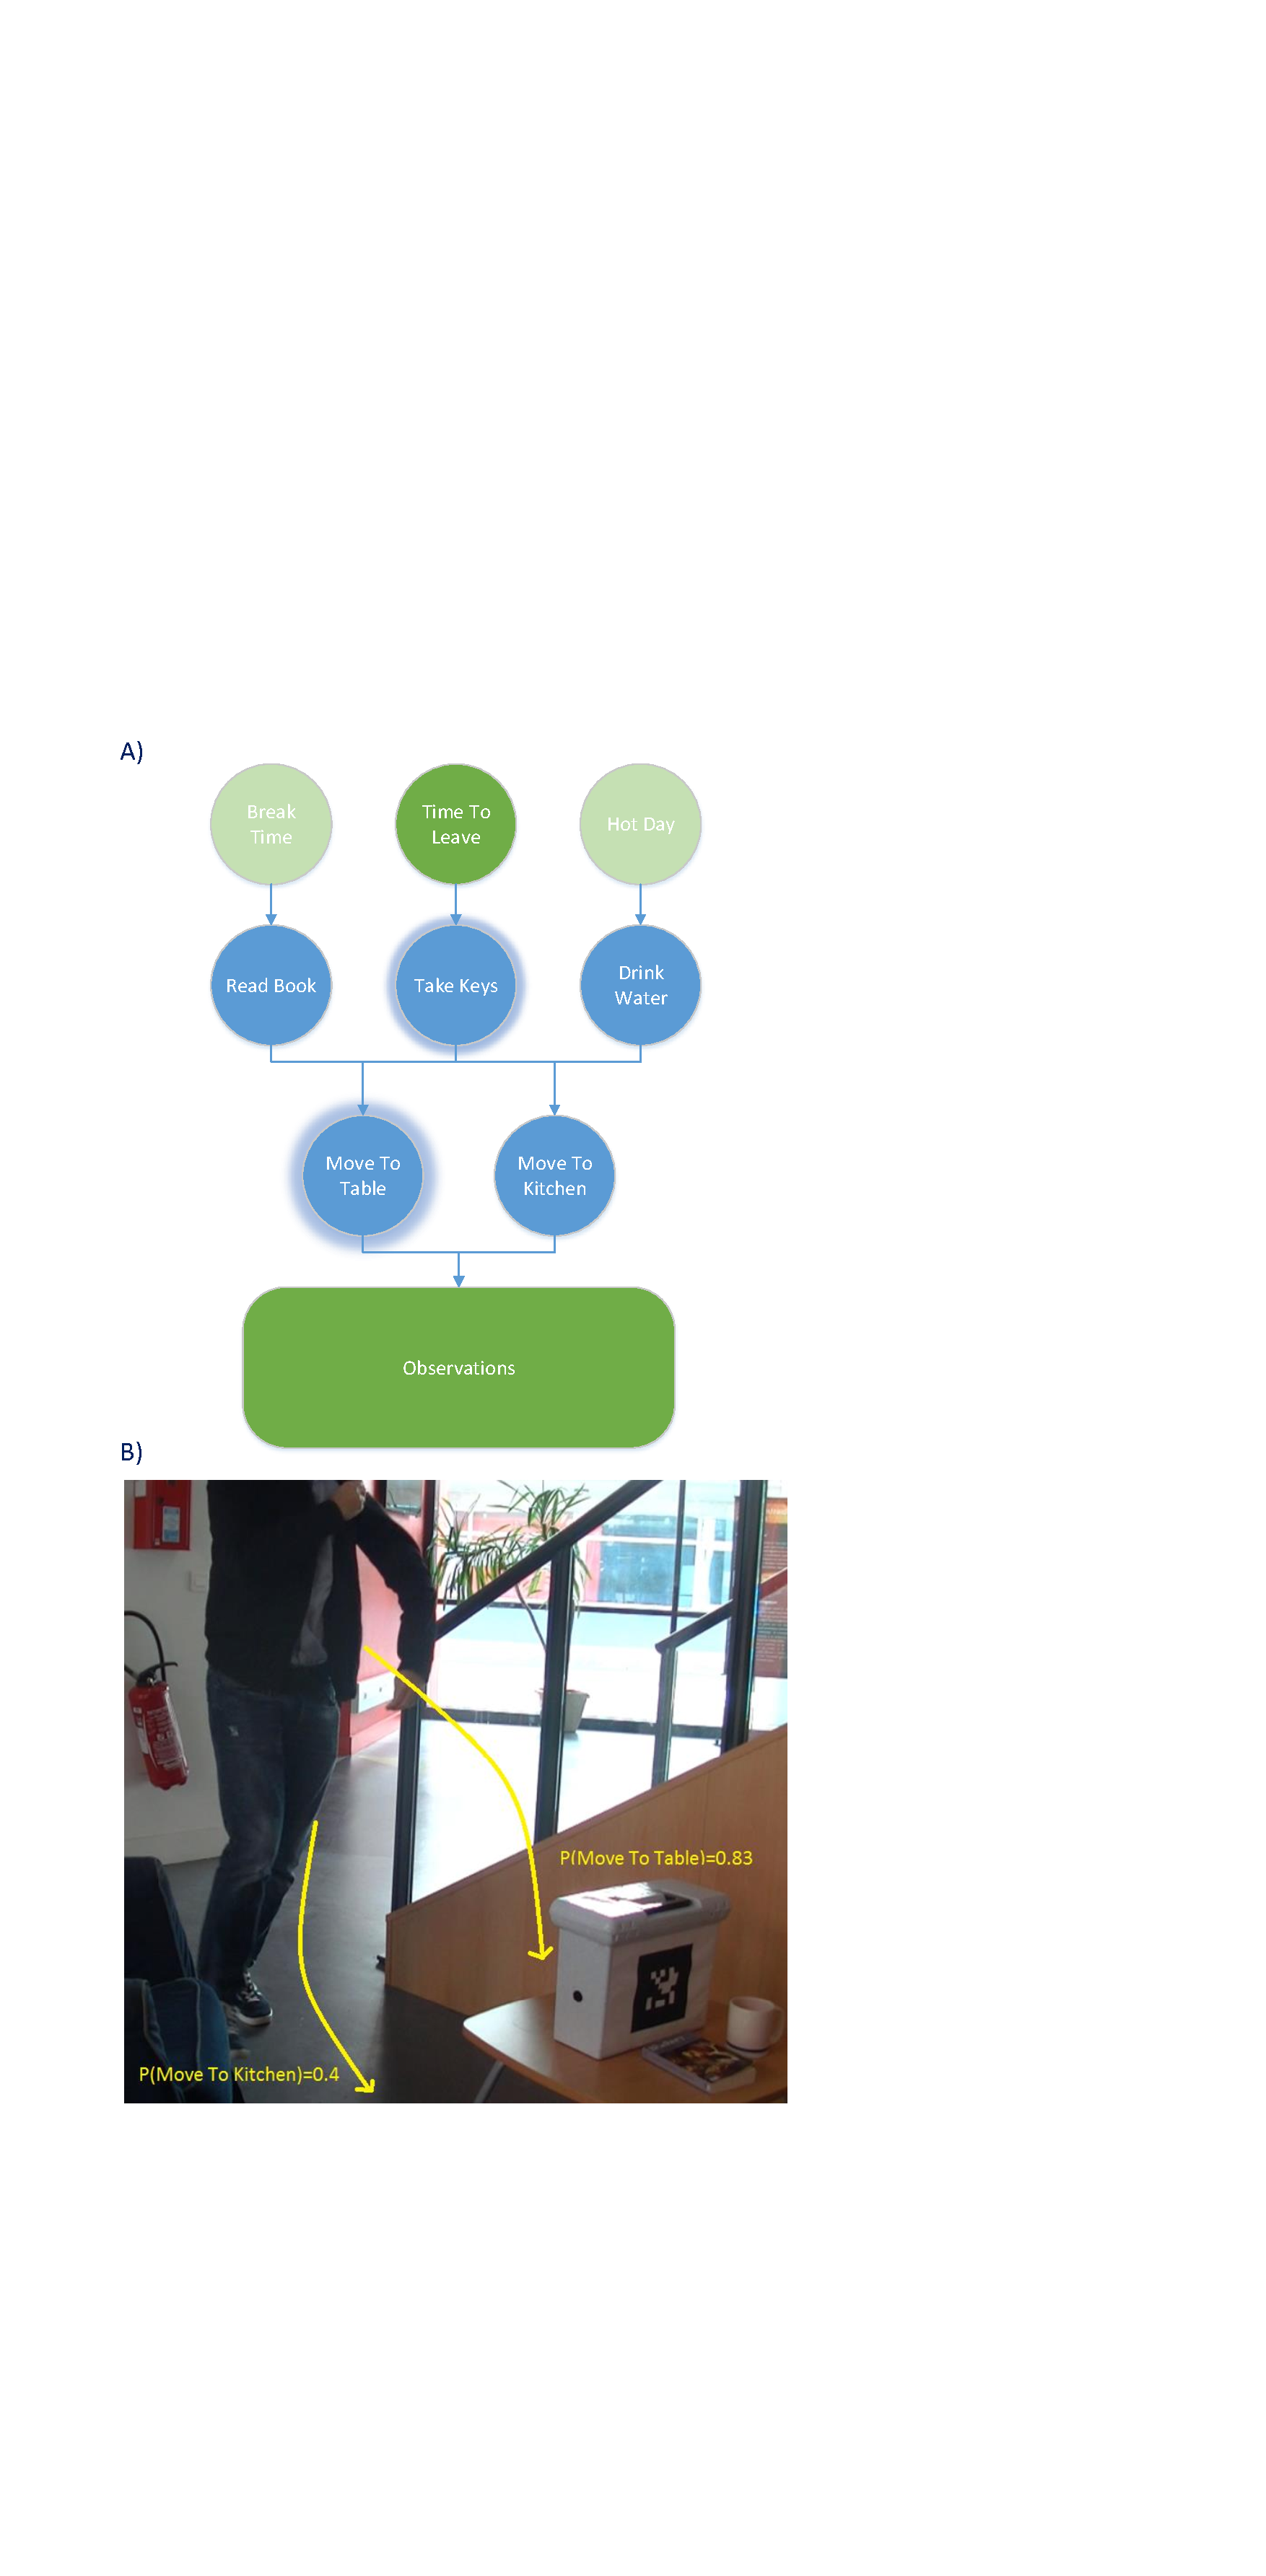
\includegraphics[trim={2cm 11cm 11cm 17cm},clip,scale=0.45]{img/situation_assessment/cookieScenario.pdf}
	\caption{A scene from our experiment. The yellow arrows show possible actions and their associated probabilities. The diagram represents the current IG. Green circles represent evidence nodes and blue circles other nodes. For the Context Nodes (top of the graph), we represented nodes with a false value as greyed out, and nodes with a true value as green. The most likely nodes in the graph are represented with a glowing effect. The observation nodes where compressed in a single block to simplify the diagram}
	\label{fig:situation_assessment-intention_graph}
\end{figure}

\subsection{From Contexts to Intentions}
We introduce a set of contexts in our domain. We consider as context any information that can be used to characterize and motivate an intention \cite{abowd1999towards}. We model a context  as a property, which can assume different values and influences the probability of a user having a particular intention. For example, we imagine that a human is more likely to be cooking at dinner time, or to drink a hot mug of tea on a cold day.

Contextual nodes can directly influence one or more Intention nodes. In this work, we chose to learn these conditional dependencies from humans, as explained in section \ref{situation_assessment-experiments}.

\subsection{From Intentions to Actions}
\label{sec:situation_assessment-action_evaluation}
To understand how actions are linked to intentions the robot needs to answer the following question: what actions would a human take, in this situation, given his belief of the world, in order to achieve its intention?
Our idea is based on the principle of rationality \cite{Dennet1989}, which states that agents tend to choose the most efficient actions, taking into account their beliefs about the world, in order to achieve their desires.

In \cite{Blakemore2001}, the authors explain that "the attribution of intentions to actions might rely on simulating the observed action and mapping it into representations of our own intention". We represent this idea by providing the robot with a set of planning models. Each one of these planning models is related to an intention, and represents all the known plans to achieve its linked goal. In this way, we can estimate how much the current human actions are compatible with the plans related to an intention.

In our implementation, for each intention known by the robot, we will create an associated Markov Decision Process (MDP), to represent all the possible plans associated to this intention. After solving the set of MDPs we will use the calculated action value function \(Q(s,a)\), to create conditional dependencies between Intention and Action nodes in the IG. Let's start by defining \(P(a|I_i=1)\), the probability that action $a$ will be performed if intention $I_i$ is true. We model this probability as \(P(a|I_i=1)=\frac{Q_i(s,a)}{\sum_b(Q_i(s,b))}\), where we normalize the value function $Q_i(s,a)$ for intention $i$ and action $a$ in the human's belief state $s$, over the value function $Q_i(s,b)$ calculated on all the monitored actions $b$. We can extend this calculation to the case where a generic number of intentions are true to compute the probabilities of action nodes: \(P(a|I_1,I_2,...,I_m)=\frac{\sum_{i:I_i=1}Q_i(s,a)}{\sum_b\sum_{i:I_i=1}Q_i(s,b)}\).

The key idea in this problem is to use the human's belief state as input for the MDPs' value functions. In this way we are using perspective taking at a planning level as the human action is consistent with his intention in his own belief state but may be irrelevant in the real world (e.g. in case of wrong belief).

Our idea is similar to \cite{karami2010human}, where human intentions are estimated using a POMDP and a set of MDPs, that simulate human policies related to different intentions. In this work we use a BN instead of a POMDP, which allows us to separate the mechanisms used for inference and for the robot's actions. Also, we improve the recognition process by including the belief state of the human.

\subsection{From Actions to Observations}
Intentions will be inferred from human actions, so the robot needs to monitor their execution. For each Action Node we define a set of four Observations Nodes: the distance of the human's body from the action's $target$, its variation, the distance of the human's hand from the action's $target$, and its variation. The conditional dependencies of the Observation Nodes are precomputed.

\subsection{Intention and Action Inference}
\label{sec:situation_assessment-intention and action inference}
We assume, in this work, that at each moment a human can only execute a single action, and the robot will react only on his most likely intention. The most likely action and intention are inferred from the BN in the following way. We call $P(n)$ the inferred probability of a node $n$, $B(n)$ the set of brothers of $n$ (that is, nodes on the same layer), and $\delta_1$, $\delta_2$ two thresholds. The robot infers that an action has been realized, or that a human has an intention following these rules: 
\begin{itemize}
\item  \(P(n_i)>\delta_1\) 
\item  \(\forall b \in B(n_i): P(n_i)>P(b)+\delta_2\), where $n_i$ is the node associated to the interested intention or action.
\end{itemize}

When the robot infers that an action has been performed, it updates the world state with its $postconditions$, triggering an update on the beliefs of all present agents. The current human intention is recorded in the Database, in order to be used by the Goal Manager.


\section{Experiments and Discussion}
\label{sec:situation_assessment-experiments}
\subsection{Case Study}
Evaluating the capacity of the system to estimate human intentions is not easy, since intentions are not directly observable. A possible solution, as shown in \cite{baker2014modeling}, is comparing the estimation of human intentions, performed by other humans, with the predictions of our system. In order to perform this comparison we created a user study where we showed participants several videos, asking them to estimate the likelihood of a set of intentions for each video, and collected their results. 

We performed an equivalence test, comparing users' intentions predictions with those of the robot, following the two one-sided tests (TOST) approach. We choose as a threshold for equivalence the standard deviation $\sigma$ of the users' answers. The idea behind this choice is that, if the robot's answers are closer than a standard deviation to the average human answers, its predictions are comparable to an average human answer from our user group. 

We defined our hypothesis as follow: 
\begin{itemize}
\item $H_0$: $\mu_{hi}-\mu_{ri}\leq-\sigma_{hi}$ OR $\mu_{hi}-\mu_{ri}\geq\sigma_{hi}$ 
\item $H_A$: $-\sigma_{hi}<\mu_{hi}-\mu_{ri}<\sigma_{hi}$  
\end{itemize}
where $\mu_{hi}$ and $\mu_{ri}$ are the human average and the robot's answer for test $i$, $\sigma_{hi}$ is the variance of the human answers for test $i$.

We performed tests to evaluate: a) prediction in absence of clues, b) prediction in the presence of contextual clues, c) prediction in the presence of belief state clues.

We built a household environment with a fixed set of furniture: a \textit{Kitchen Shelf}, a \textit{Table}, a \textit{Sofa}, and a \textit{Chair}. In this environment, we created two scenarios, composed by several tests, with two agents, \textit{Max} and \textit{Bob}, performing different actions. Each scenario contained a set of objects, and a constrained set of intentions. For the tests related to belief states, we start by showing the users and the robot a specific sequence of events, allowing them to build a mental model of the agents. We will describe in details the two scenarios and the relative tests.

\subsubsection{Cookie Scenario}
\begin{itemize}
\item Objects: a \textit{Cookie Box}, a \textit{Mug}, and a \textit{Bottle of Water} were placed on the \textit{Table}, close to each other. A pack of \textit{Cookies} was placed on the \textit{Kitchen Shelf}. The \textit{Cookie Box} could contain, or not, \textit{Cookies}.
\item Intentions: \textit{Eating a Cookie}, \textit{Drinking Water}, \textit{Reading the Book}.
\item Tests:
\begin{itemize}
	\item \textit{No Clues}: \textit{Max} approaches the \textit{Table}.
    \item \textit{Contextual Clues}: \textit{Max} approaches the \textit{Table} commenting on the warmth of the day.
	\item \textit{Divergent Belief Max}: \textit{Max} approaches the \textit{Table}.
	\item \textit{Divergent Belief Bob}: \textit{Bob} approaches the \textit{Table}.
\end{itemize}
\item  \textit{Divergent Belief Event}:  \textit{Max} and \textit{Bob} are chatting on the \textit{Sofa}. Max eats the last \textit{Cookie} from the \textit{Cookie Box} before closing it and leaving. While \textit{Max} is away, \textit{Bob} takes \textit{Cookies} from the \textit{Kitchen Shelf}, fills the \textit{Cookie Box} with them, and closes it, before leaving.
\end{itemize}

The \textit{Divergent Belief Event} was shown to the users and the robot between the \textit{Contextual Clues} and the \textit{Divergent Belief Max} events. 

We deliberately included an intention, \textit{Reading the Book}, without placing a book in the visible environment, introducing a confusing element in the scenario.

\subsubsection{Keys Scenario}
\begin{itemize}
\item Objects: A \textit{Box} was placed on the \textit{Table}, that partially occluded the sight of people approaching. A \textit{Book} and a \textit{Mug} where placed behind the \textit{Box}, so that they could be seen from the sofa but not from approaching people.
\item Intentions: \textit{Taking the Mug}, \textit{Taking the Keys}, \textit{Reading the Book}.
\item Tests and Events:
\begin{itemize}
\item \textit{No Clues}: \textit{Max} approaches the \textit{Table}.
\item\textit{Contextual Clues}: \textit{Max} approaches the \textit{Table} in a hurry, while putting on a coat.
\item \textit{Divergent Belief Max}: \textit{Max} approaches the \textit{Table} in a hurry, while putting on a coat.
\end{itemize}
\item \textit{Divergent Belief Event}: \textit{Max} is sitting on the \textit{Table}, drinking from the \textit{Mug}, while having the \textit{Keys} in his hands. His phone rings, so he drops the \textit{Keys} and the \textit{Mug} on the \textit{Table}, behind the \textit{Box}, and leaves the room. While \textit{Max} is away, \textit{Bob} comes and sits on the \textit{Sofa}, reading a \textit{Book}. When he sees the \textit{Keys}, he takes them, places the \textit{Book} on the \textit{Table}, and leaves.
\end{itemize}

The \textit{Divergent Belief Event} was shown to the users and the robot between \textit{Contextual Clues} and the \textit{Divegent Belief Max} events.

\subsection{User Study}
We built an online user study, where we presented videos related to the tests and events of the two scenarios to users, who had to evaluate the likelihood of each intentions of the scenario
on a five-level Likert scale. The user study was conducted in three languages, with users living in two different countries\footnote{A version of this user study was provided at http://goo.gl/forms/YiuFHnF63c}. We collected answers from 78 adults, performed an average, and converted them to percentile scores, in order to compare them with the robot's predictions.

Looking at users' answers (Fig. \ref{fig:situation_assessment-user_study_results}), we can see that, in the absence of clues, people rated similarly the two intentions related to visible objects. Contextual clues had the highest influence on users' ratings. This is particularly visible in the \textit{Contextual Clues} test of the \textit{Keys Scenario}, where users chose as the most likely intention \textit{Take Keys}, even if no keys were visible in the video. Divergent beliefs also influenced users decisions, but not as strongly as context. The strongest responses, over all, where given by the \textit{Divergent Belief Max} test on \textit{Keys Scenario}, which uses both divergent belief and contextual information.

\subsection{Robot implementation}
At the start of a scenario the robot scanned the environment, building a model of its world state. With our perception capacities, we can't detect if the cookie box is full or empty, and so we consider it as full at the start of a test, and update its value using the $postconditions$ of inferred human actions. We consider the box as empty when we infer that a human has taken a cookie from inside, and as full when we infer that a human has put a cookie in it.

We built different IGs for the scenarios. Each test had a different graph, related to it's main agent. We considered three different Context Nodes for these IGs: Hot Day, true when the day is particularly warm; Break Time, true when the agents are taking a pause; Time to Leave, true when it's late in the day, and the humans usually leave work and return home.

As previously said, we chose to follow \cite{Liu2014} in order to learn the link between Contexts and Intentions. We created a second user study with 15 users, in which we presented a set of 5 scenarios, each one related to one of the intentions of our tests. For each scenario we asked the users to rate the perceived link, on a five-level Likert scale, between the intention and our three contexts. We averaged users' answers and calculated the conditional probabilities between context nodes and intention nodes from these averages.


In the \textit{Cookie Scenario} the graph for the tests is constructed from the following nodes:
\begin{itemize}
\item Context Nodes: \textit{Hot Day}, \textit{Break Time}, \textit{Time to Leave}
\item Intention Nodes: \textit{Fill Cookie Box}, \textit{Eat Cookie}, \textit{Drink Water}, \textit{Read Book}.
\item Action Nodes: \textit{Move to Table}, \textit{Move to Kitchen}.
\item Observation Nodes: distance of the agent body and hand to each action's associated \textit{interesting points}.
\end{itemize}

We introduce the \textit{Fill Cookie Box} intention, not present in the human test, to allow the robot to detect when Bob fills the \textit{Cookie Box} during the \textit{Divergent Belief Event}.

Our robot doesn't have speech recognition capacities. We simulated this capacities, and set Context Nodes to plausible values, that could be extracted by watching the videos. For the \textit{Contextual Clues} test, we set the value of \textit{Hot Day} to true (since Max is commenting about the temperature), and \textit{Break Time}, and \textit{Time to Leave} to false (since no data in the video points to one of these contexts being true. Max and Bob seem to have taken a break from work before the other events are shown, in the Divergent Belief Event).
%Our robot doesn't have speech recognition capacities. and for \textit{Contextual Clues} test, set the value of \textit{Hot Day} to \textit{true}, and the value of \textit{Break Time} to \textit{false}, i.e. the robot knows that it is not the usual time for the agents to take a break.

\textit{Divergent Belief Event}, \textit{Divergent Belief Max}, and \textit{Divergent Belief Bob} were showed sequentially to the robot, which updated the agents' mental models and created new IGs accordingly. During the \textit{Divergent Belief Event} several IGs need to be created with different action and observation nodes, to follow the sequence of actions by the two agents. For example, when \textit{Max} leaves the room, \textit{Bob} has the possibility to execute the actions \textit{Take Mug}, \textit{Take Water Bottle}, \textit{Open Cookie Box}, \textit{Move to Kitchen Shelf} or \textit{Leave Room}. Intention and Context nodes remains the same in all the IGs of the scenario.


The \textit{Keys Scenario} has a similar IG, with the following differences.
\begin{itemize}
\item Context Nodes: \textit{Hot Day}, \textit{Break Time} and \textit{Time to Leave}.
\item Intention Nodes: \textit{Drink Water}, \textit{Take Keys}, \textit{Read Book}.
\end{itemize}

Action Nodes and Observation Nodes are the same as the previous scenario, and follow the same ideas during the \textit{Divergent Belief Event}. An example of IG used in the tests can be seen in Fig. \ref{fig:situation_assessment-intention_graph}. For the \textit{Contextual Clues} and \textit{Divergent Belief} test, we set the \textit{Time to Leave} context value to \textit{true} (since Max is putting a coat and seems in a hurry), and other context node values to \textit{false}. Using the component described in the previous sections, and these IGs the robot was able to obtain predictions from the user actions.

\subsection{Discussion}
\label{sec:discussion}
We performed TOST tests for each intention in the scenarios, comparing the humans' answers with the robot's, for a total of 21 tests.

We calculated p-values and performed our tests using a significance value $\alpha=0.05$.

Analyzing the results of our equivalence tests, shown in Fig. \ref{fig:situation_assessment-user_study_results}, produces some interesting information. 1) The behavior of our system is often close to human capacities. 19 tests out of 21 passed our requirements for significance level, often with very low p-value scores. 2) Context and Divergent Belief are necessary. A system without these skills would only have been able to model properly the \textit{No Clues} cases. 3) There are still some missing aspects in our system. We failed to reject the null hypothesis for two tests. In \textit{Divergent Belief Bob} users rated higher the \textit{Eat Cookie} intention than the \textit{Drink Water} intention, possibly because they thought that since \textit{Bob} filled the \textit{Cookie Box} he may want to eat a \textit{Cookie}. This makes us think that humans use deep temporal reasoning to evaluate intentions, considering the whole history of actions performed by agents.  

 \begin{figure}[h!]
	\centering
	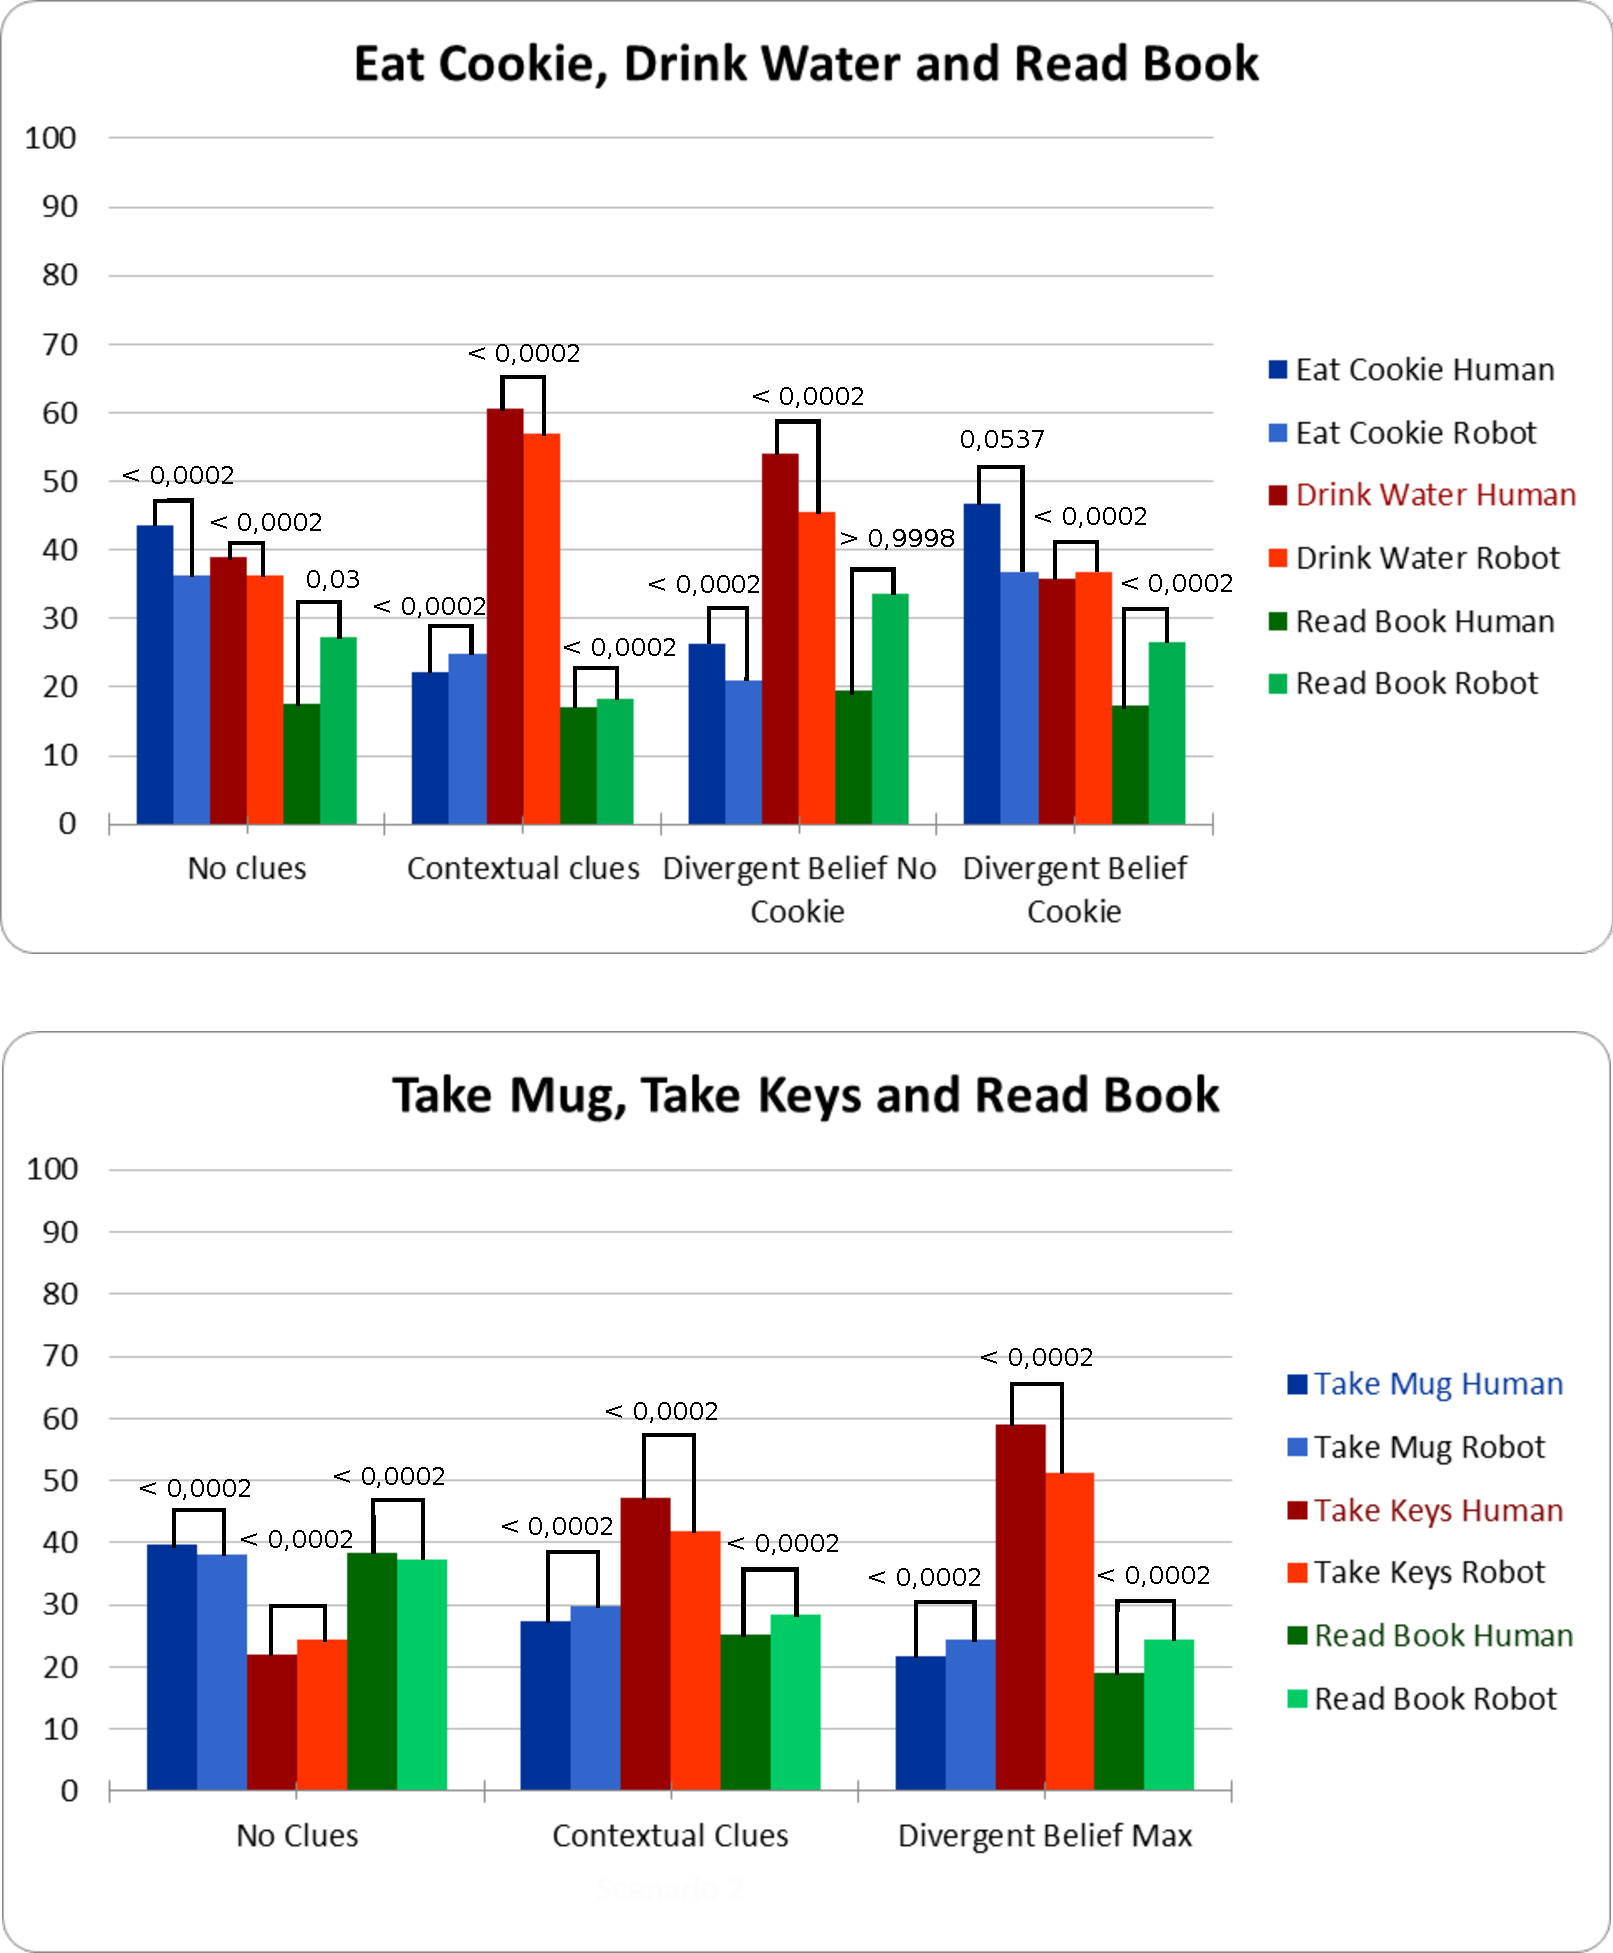
\includegraphics[clip,scale=0.32]{img/situation_assessment/pvalues1.pdf}
	\caption{Experiment results. Results from the two scenarios are represented as graphs. Intentions, as estimated by the humans and the robot, are represented by different colors, as shown in the legend of the graphs, with estimations of the same intention by the robot or the human placed in adjacent position. Each column represents the likelihood of an intention, expressed as a percentile score. P-values from the equivalence tests are shown, linking the estimation of an intention by the humans and by the robot.}
	\label{fig:situation_assessment-user_study_results}
\end{figure}



 
\chapter{Inferring Human Intention and Reacting} % Main chapter title

\label{chapter:intention} % Change X to a consecutive number; for referencing this chapter elsewhere, use \ref{ChapterX}

\lhead{Chapter 3. \emph{Intention Recognition}} % Change X to a consecutive number; this is for the header on each page - perhaps a shortened title


\section{Introduction}
Another crucial skill to interact with humans is recognizing others' actions and goals. This process is is directly linked to modeling humans' beliefs, since, as explained by \cite{byom2013theory} ``as humans, we generally believe that others act in ways that are consistent with their beliefs and goals". 

The recognition of human activities is an important topic in computer science research, which can be studied at different levels. Anticipating human actions and movements allows the robot to adapt its behavior and proactively help humans, as studied in \cite{koppula2013anticipating}. 

Sequences of actions can be linked to plans, a well-known topic called plan recognition. Several approaches have been studied in this domain using, for example, classical planning \cite{ramirez2009plan}, probabilistic \cite{bui2003general} or logic techniques \cite{singla2011abductive}.

Other approaches that can be used to estimate the intention of a human are Interactive Partially Observed Markov Decision Processes (I-POMDP) and Inverse Learning. I-POMDP  \cite{gmytrasiewicz2004interactive} offer a rich framework that extends Partially Observed Markov Decision Processes (POMDP) in a multi-agent setting. Inference in these models can be extremely complex, but there have been attempts at solving this issue, like in \cite{doshi2009monte,hoang2013interactive}. 

Inverse Reinforcement Learning \cite{ng2000algorithms} formulates the problem of computing an unknown reward function of an agent after observing his behavior. This strategy has been applied, with Bayesian Networks (BN), in \cite{Nagai2015}, in order to learn the mental model of another agent, and choose appropriate actions for a relationship building task. A linked approach is inverted planning, which has been applied in a bayesian framework in \cite{baker2009action}  for human action understanding.

The use of contextual information can be used to further disambiguate complex situations. \cite{Liu2014} shows a system using BNs to understand users' intentions with an emphasis on contextual information. This BN is constructed using object affordances nodes (e.g. a cup can be washed or used for drinking), context nodes (e.g. it's a hot day, the cup was recently used), and intention nodes (e.g. drinking from a cup or washing it). The causal links between contexts and intentions are learnt through a user study, which uses an online questionnaire where participants need to rate the strenght of the connection betwen an intention and a context. The work does not study how to adapt this BN to complex plans, composed by sequences of actions.

It is very important to consider humans' beliefs when estimating their intentions. In a dynamic environment, agents can execute actions, modifying the state of the world without other agents being able to perceive the changes. Let us imagine a scenario. Bob comes back home from work and would like to relax while reading. He lays down on a sofa with a book, and reaches to a nearby table to grab his glasses. He does not know that his wife, during the day, moved the glasses to another room. If we would ignore Bob's beliefs on the world (i.e. he does not know that the glasses are not on the table) we could infer that, for example, Bob would like a drink while he is sitting on the sofa, or the tv remote controller. If, instead, we would know that Bob thinks his glasses are on the table (and we would use other contextual information perhaps, like Bob's habitudes) we would be able to correctly infer Bob's current intention, that is, taking his glasses, and warn him that they are not there, perhaps even fetching them for him. 

In robotics, an interesting framework that considers this issue is the Bayesian Theory of Mind \cite{baker2014modeling}, used to represent the inference process of an observer looking at another agent's behaviors. The acting agent is modeled as a POMDP, whose richness is able to represent its possible beliefs about the world. The observer's process is modeled as a DBN, built starting from the agent's POMDP but considering his reward function (that represents his desires) as hidden. The system has been tested against some alternative models and compared, in user studies, with human capacities, to understand how well it models theory of mind. Since the models used are quite complex, scalability in the model could be an issue. Also, the study is focused on a single-agent scenario, and does not consider collaborative problems.

Let us examine the two simulation-based systems that we already presented in the previous section, HAMMER ~\cite{demiris2007prediction}, and the architecture of \cite{BreazealGB09}, and see how these cognitive architectures are able to infer actions and intentions.

The HAMMER system is organized with couples of inverse and forward models.  Inverse models receive as input the goal and state of the system, producing the motor commands which are needed to achieve the goal. Forward models, instead, receive as input motor commands and compute the predicted future state. When these two models are linked, the forward model receives as input the motor commands produced by an inverse model. This link can form a loop, with the output of a forward model returning to its inverse model, which can adjust a range of parameters if the predicted future state does not match exactly the desired state. These models can be organized in parallel schemas and used to recognize actions performed by a demonstrator. 

In this case, the demonstrator's current state, as perceived by the robot, is fed in the inverse models, which in turn sends their output to their forward models. The state predicted by the forward models are compared with the demonstrator's state at the next time step. This comparison produces a score, which can be used to infer the most likely action performed. 

Forward and inverse models can be organized in hierarchical schemas, to infer actions and plans. The complexity of these schemas could be quite significant, particularly when trying to recognize a goal which can be achieved in many different ways, depending on the context. 

\cite{BreazealGB09} uses a similar ideas, where the all the possible robot movements are represented as a graph of connected poses, with arcs representing possible transitions between the poses. This graph is used both to represent the robot's movements and to map observed trajectories. Tasks are represented as schemas, which can be organized in sequential and hierarchical structures to represent complex goals.

 When trying to infer an agent's intention the robot looks for a schema whose motor action matches the observed activities of the agent. After that, the schema is traversed in reverse in order to try to determine the real intention. The system is not able to deal with ambiguities, and this algorithm stops if it comes to a point where there is more than a possible explanation for the current behavior. 

An example of non simulation-based system in this topic can be seen in \cite{talamadupula2014coordination}. This architecture is used to coordinate human-robot teams, based on intention recognition and belief modeling. Creating and maintaining beliefs is handled using the strategy explained in ~\cite{scheutz2013computational}, presented in the previous subsection. Prediction of other humans intentions' is based on the plan recognition algorithm of \cite{ramirez2009plan}. While this algorithm uses efficient replanning to increase its efficiency, in complex domains, where the users have many different strategies to achieve a goal, the system would need to execute frequent replans to infer the actual strategy chosen by the user, which can be expensive.


\section{Intention and Action Inference}
\label{sec:situation_assessment-intention_recognition}
Understanding what others are doing is an important skill for a robot partner. We have designed a module that is able, through inference, to recognize human actions and connect them to possible intentions. Actions and intentions are evaluated with perspective taking using the humans' belief models, and further disambiguated by taking into account the current context.

In order to perform this reasoning, we will provide the following information to the robot: a list of known contexts, a list of known intentions, a list of known actions, a set of observations of human actions, and a belief model of humans and of the robot itself.

We introduce a simplification in our model: at each time step, a human can execute only one action and has only one intention, decreasing the ambiguities in the inference process.

We propose, as central model used for intention estimation, a framework based on BNs. We call our implementation of BN an Intention Graph (IG).
An IG is linked to a specific human, and composed by the following layers of nodes:
\begin{itemize}
\item Context Nodes: these nodes represent contextual information, modeled as boolean variables (e.g. HotDay, ColdDay).
\item Intention Nodes: these boolean nodes represent the set of possible intentions. Each intention can conditionally depend on several contexts.
\item Action Nodes. This is the set of human actions whose preconditions are satisfied when the IG is created. Each of these nodes is conditionally dependent on all the intention nodes. 
\item Observation Nodes. We associate to each action a different set of observation nodes, that depend conditionally on the associated action node. For example, the distance of a human from the \textit{target} of an action can be an Observation Node.
\end{itemize}

In a typical usage, the robot will create, for each monitored human, an IG, formed by the Context and Intention Nodes, which we consider statically known by the robot, and a variable list of Action and Observation nodes, which depends on the human's belief model. The robot will create action nodes for each known action whose $preconditions$ are satisfied in the human's belief model, and their related Observation Nodes. These IGs will be updated every time that an agent performs an action, creating and removing Action and Observation nodes, depending on the state of the world after the action was performed.

When monitoring a human, we set Context Nodes and Observation Nodes as \textit{evidence}, considering them observable by the robot. These information will allow us to have a good estimation of the most likely actions and intentions of the human, as explained in subsection \ref{sec:situation_assessment-intention and action inference}. 


An example of IG, taken from an experiment, can be seen in figure \ref{fig:situation_assessment-intention_graph}. In the following paragraphs, we will explain the role of these layers of nodes, and how the conditional dependencies between them are computed. After that, we will show an example showing how an IG is created and updated following a sequence of human actions, and how the robot is able to use it to infer the most likely human intention.

 \begin{figure}[ht!]
	\centering
	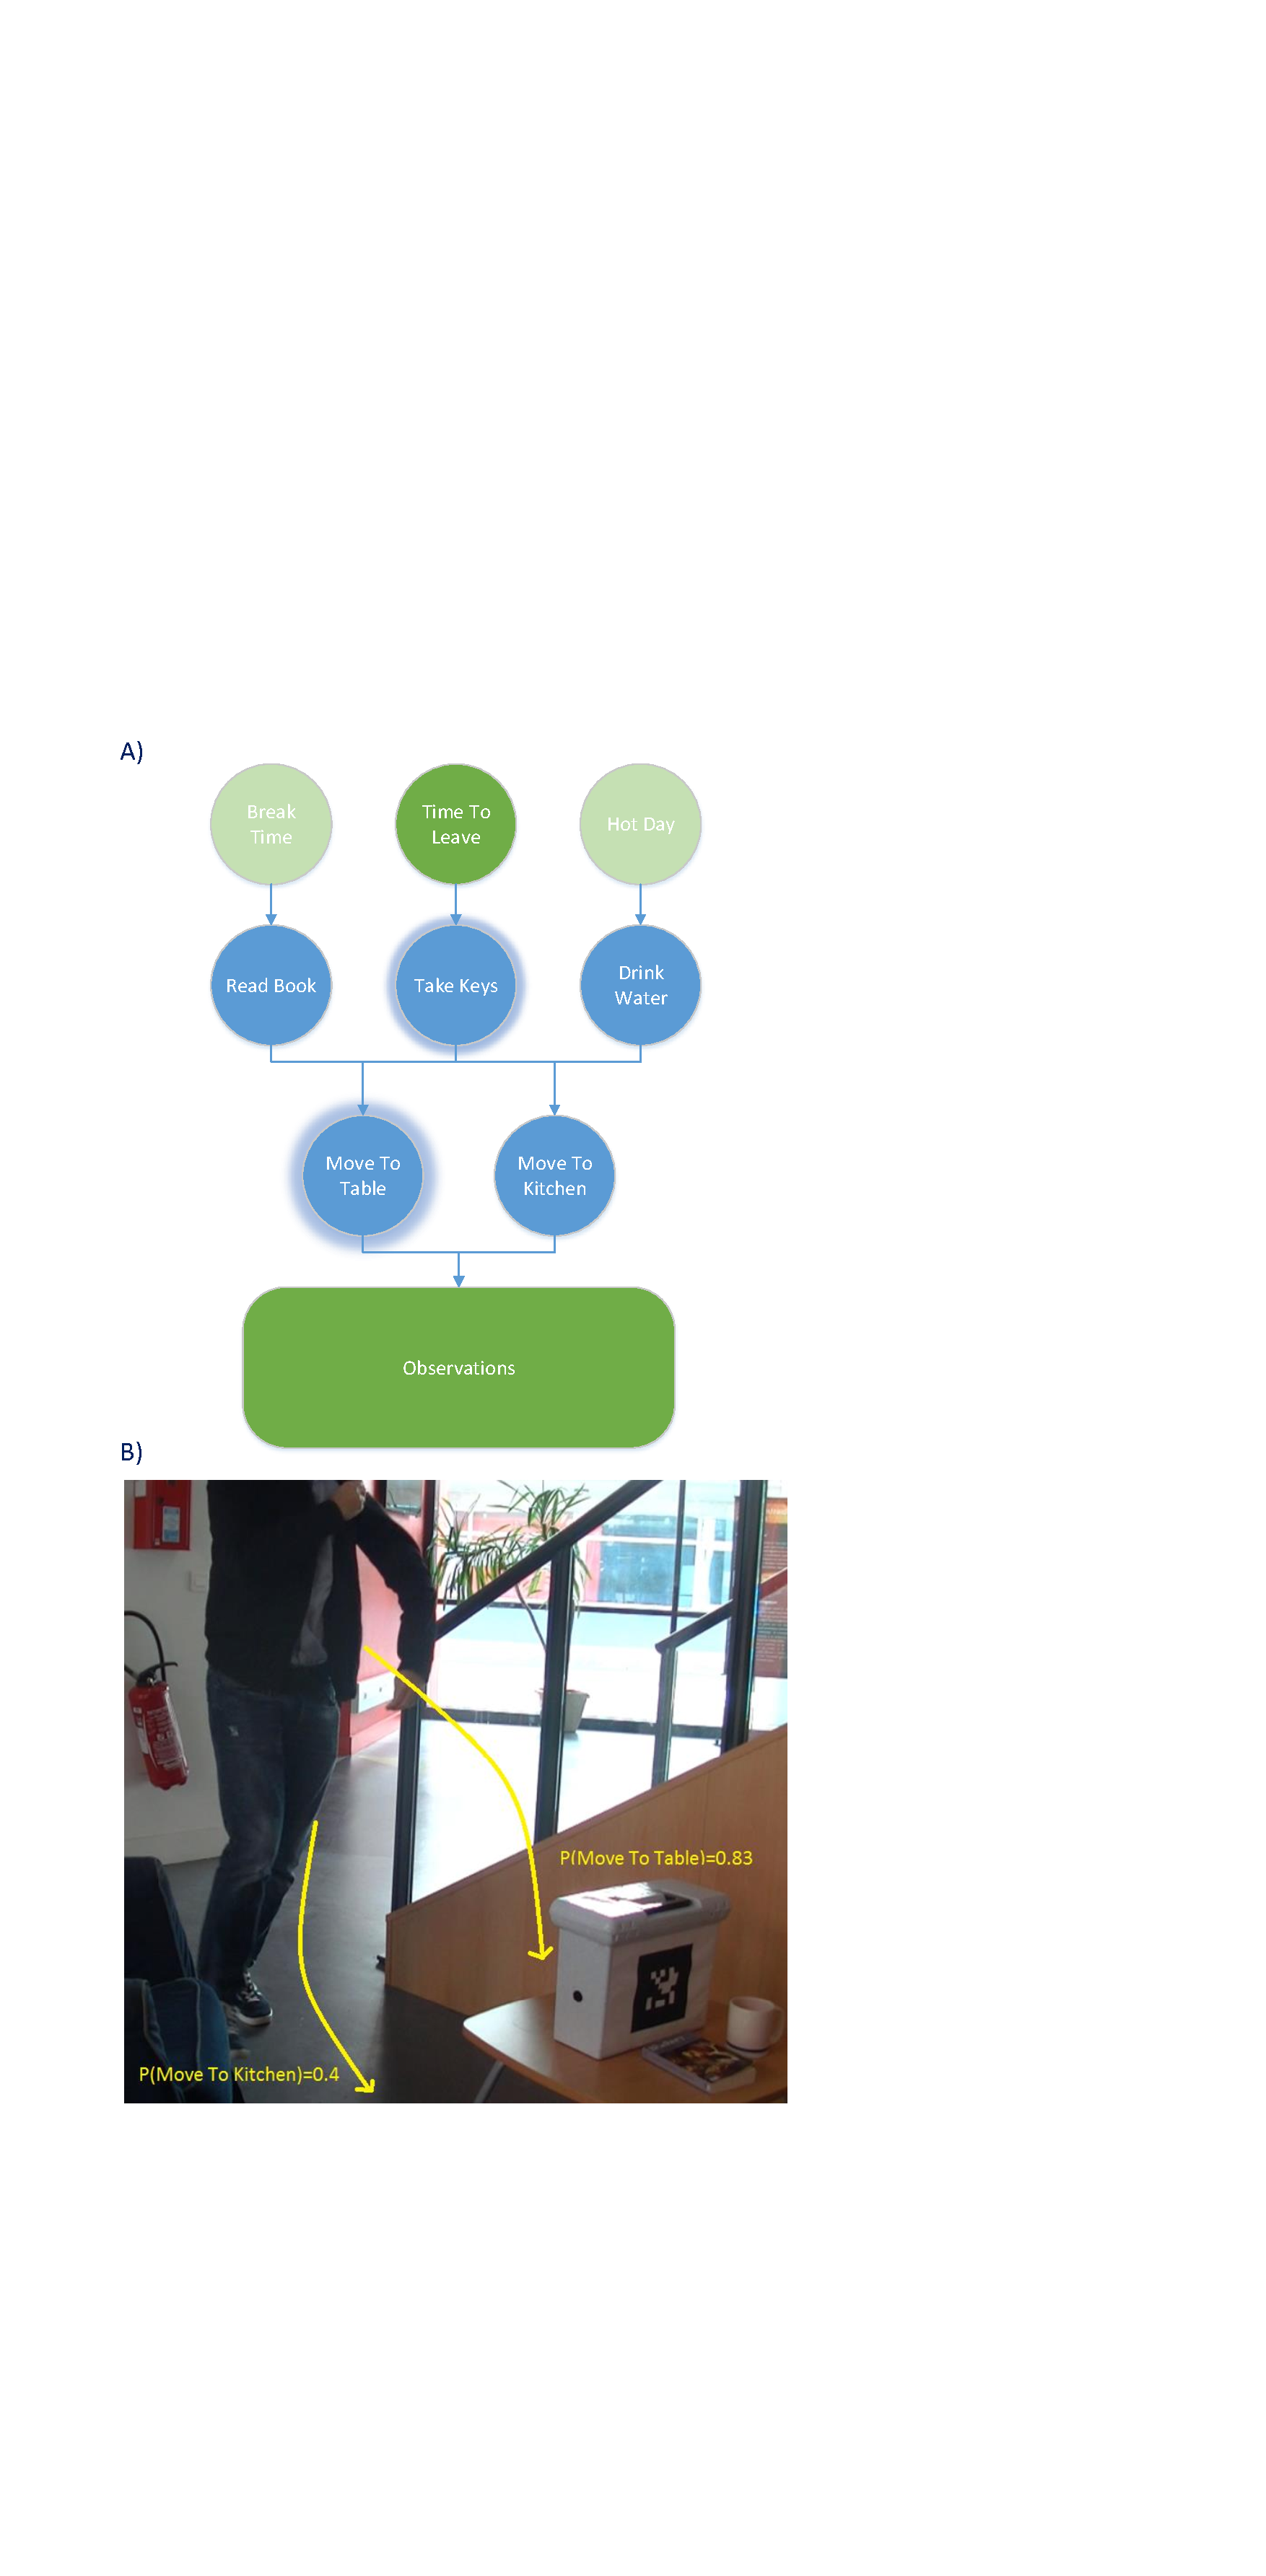
\includegraphics[trim={2cm 11cm 11cm 17cm},clip,scale=0.45]{img/situation_assessment/cookieScenario.pdf}
	\caption[Intention Graph]{A scene from our experiment. The yellow arrows show possible actions and their associated probabilities. The diagram represents the current IG. Green circles represent evidence nodes and blue circles other nodes. For the Context Nodes (top of the graph), we represented nodes with a false value as greyed out, and nodes with a true value as green. The most likely nodes in the graph are represented with a glowing effect. The observation nodes were compressed in a single block to simplify the diagram}
	\label{fig:situation_assessment-intention_graph}
\end{figure}

\subsection{From Contexts to Intentions}
We introduce a set of contexts in our domain. We consider as context any information that can be used to characterize and motivate an intention \cite{abowd1999towards}. We model a context  as a fact, which can assume different values and influences the probability of a user having a particular intention. For example, we imagine that a human is more likely to be cooking at dinner time, or to drink a hot mug of tea on a cold day.

Contextual nodes can directly influence one or more Intention nodes. In this work, we chose to learn these conditional dependencies from humans, as explained in section \ref{sec:situation_assessment-experiments}.

\subsection{From Intentions to Actions}
\label{sec:situation_assessment-action_evaluation}
To understand how actions are linked to intentions the robot needs to answer the following question: what actions would a human take, in this situation, given his belief of the world, in order to achieve its intention?
Our idea is based on the principle of rationality \cite{Dennet1989}, which states that agents tend to choose the most efficient actions, taking into account their beliefs about the world, in order to achieve their desires.

In \cite{Blakemore2001}, the authors explain that ``the attribution of intentions to actions might rely on simulating the observed action and mapping it into representations of our own intention". We represent this idea by providing the robot with a set of planning models. Each one of these planning models is related to an intention, and represents all the known plans to achieve its linked goal. In this way, we can estimate how much the current human actions are compatible with the plans related to an intention.

In our implementation, for each intention known by the robot, we will create an associated Markov Decision Process (MDP), to represent all the possible plans linked to this intention. After solving the set of MDPs we will use the calculated action value function \(Q(s,a)\), to create conditional dependencies between Intention and Action nodes in the IG. We define \(P(a|I_i=1)\), the probability that action $a$ will be performed if intention $I_i$ is true, as as:
\begin{equation}
 P(a|I_i=1)=\frac{Q_i(s,a)}{\sum_b(Q_i(s,b))}
\end{equation}
  where we normalize the value function $Q_i(s,a)$ for intention $i$ and action $a$ in the human's belief state $s$, over the value function $Q_i(s,b)$ calculated on all the monitored actions $b$. 

%   We can extend this calculation to the case where a generic number of intentions are true to compute the probabilities of action nodes: 
% \begin{equation}
%   P(a|I_1,I_2,...,I_m)=\frac{\sum_{i:I_i=1}Q_i(s,a)}{\sum_b\sum_{i:I_i=1}Q_i(s,b)}
% \end{equation}

The key idea in this problem is to use the human's belief state as input for the MDPs' value functions. In this way we are using perspective taking at a planning level, since the human action will be consistent with his intention in his own belief state but may be not optimal, irrelevant, or even dangerous in the real world (e.g. in case of wrong belief).

Our idea is similar to \cite{karami2010human}. In this work, the robot planning model is a POMDP, where the human intention is a hidden variable. The transition function for the human intention is computed starting from the action values obtained from a set of human MDPs, that simulate human policies related to different intentions. In this work, we used a BN for the inference process, instead of a POMDP. This allows us to include in a simple way more information in the inference process, such as context, and to separate the mechanisms used for inference and for the robot's actions. Also, we improve the recognition process by including the belief state of the human.

\subsection{From Actions to Observations}
Intentions will be inferred from human actions, so the robot needs to monitor their execution. For each Action Node we can define a different set of Observation Nodes, which depend on the specific actions. Typical examples are: the distance of the human's body from the action's $target$, its variation, the distance of the human's hand from the action's $target$, and its variation. The conditional dependencies of the Observation Nodes are precomputed.

\subsection{Intention and Action Inference}
\label{sec:situation_assessment-intention and action inference}
We assume, in this work, that at each moment a human can only execute a single action, and the robot will react only to his most likely intention. The most likely action and intention are inferred from the BN in the following way. We call $P(n)$ the inferred probability of a node $n$, $B(n)$ the set of brothers of $n$ (that is, nodes on the same layer), and $\delta_1$, $\delta_2$ two thresholds. The robot selects the most likely action and intention following these rules: 
\begin{itemize}
\item  \(P(n_i)>\delta_1\) 
\item  \(\forall b \in B(n_i): P(n_i)>P(b)+\delta_2\), where $n_i$ is the node associated to the interested intention or action.
\end{itemize}


To infer that an action has been performed, the robot uses an estimation of the action's probability and geometrical reasoning. For example, the robot infers that a human has taken a bottle if his hand is closer to it than a threshold $\sigma$  and the action's probability in the IG respect the previous rules. For another example, the robot infers that a human has mixed some ingredients in a bowl if his hand approaches the bowl and then leaves after some seconds, always taking into account the probability of the action in the IG.

When the robot infers that an action has been performed, it updates the world state with its $postconditions$, triggering an update on the beliefs of all present agents. The current human intention is recorded in the Database, and will be used by the Goal Management layer.

 \begin{figure}[ht!]
	\centering
	\includegraphics[scale=0.8, trim={0 4cm 0 0}]{img/situation_assessment/pick.pdf}
	\caption[Actions and world update]{The human picks an object and the robot updates accordingly the world state. The spheres surrounding objects show when the human's hand is considered to be near an object.}
	\label{fig:situation_assessment-pick}
\end{figure}


\subsection{Proactive Behaviors}
\label{subsec:situation_assessment-proactive_behaviors}
Information about the most likely intention and action will be introduced in the database, to be read by the Goal Management Layer. Based on this information, the robot can execute two different proactive behaviors: correcting the belief state of the human, and proactively helping him to achieve his task.

\subsubsection{Correcting Belief State}
Having a wrong or incomplete belief on the world state can lead agents to execute non optimal, useless, or even dangerous actions. The robot needs to detect these situations in order to warn the human. For example Greg could search for his glasses in a wrong location if he does not know that they were moved, or could touch a hot object if he does not know its temperature.

 The robot assumes that it always holds a correct belief state. Our solution uses the expected action rewards introduced in \ref{sec:situation_assessment-action_evaluation}. The idea is comparing the expected reward for performing an action according to the human and the robot's belief states. To formalize: we compare the action values \(Q_m(s_h,a_h)\) and \(Q_m(s_r,a_h)\), where $m$ is the most likely intention,  $s_h$ and $s_r$ are the robot's and human's belief state, and $a_h$ is the most likely action. If these values are not equal the human expects a different outcome from its action than what should actually happen. 

We propose a simple solution, where the robot warns the human of the detected divergent belief for that action. For example, Bob wants to drink tea from a closed, opaque bottle, which the robot knows is empty (perhaps because another agent drank the last glass), while Bob does not. When he approaches the bottle, the robot detects that his most likely intention is to drink tea. The system calculates the expected rewards from taking the bottle in the two belief models and obtains different values. The system checks the facts related to the attributes associated to the bottle in the two mental models, and extracts the differences. Using this information, the robot corrects the divergent belief, informing the human that the bottle is now empty. 

In our system, the Goal Management layer will detect these situations, by reading the Database, and choose a \textit{warn agent} goal (as will be explained in chapter \ref{chapter:goal_management}).

In a real scenarios, the human might have several divergent beliefs at the same time. While the robot could inform the human as soon as it detects a divergent belief, it would risk overloading the human with unneeded information. For example, Greg might not know that his wife drank a mug of coffee or moved the remote control to the table, but maybe he will not need these information in the near future. We chose, with this approach, to give information about a divergent belief only when it risks impacting the action of a human.

\subsubsection{Performing a part of the plan}
There are situations in which the robot should help the human achieve its goal by physically acting. The Goal Management layer will consider new inferred intentions as possible goals for the robot, and will communicate with the Plan Production and Management layer to achieve them, as explained in chapters \ref{chapter:goal_management}, \ref{chapter:plan_management}, and \ref{chapter:plan_execution}. 


\subsection{Intention Graph Example}

\subsubsection{Scenario}
We will now show an example of use of an IG. We start by defining a scenario with a human, Greg, and two possible intentions: drinking water and reordering a table, by moving all the objects on top of it to the kitchen. We set three different locations: a \textit{table}, a \textit{shelf}, and a \textit{kitchen}. We consider two objects: a \textit{glass} and a \textit{bottle}. The \textit{bottle} and the \textit{glass} can contain water, but the \textit{bottle} is opaque and Greg can not observe if there is water or not in it. Of course, this scenario is not realistic and is chosen just to illustrate the IG. In a real situation Greg would notice that the bottle is empty when taking it, because it would be too light, or when opening it.
At the start of the scenario, Greg is at the \textit{shelf}, the \textit{bottle} and \textit{glass} are on the \textit{table}, and the they are both empty. 

We set a situation of divergent belief, where Greg does not know that the bottle is empty, but the robot has this information. 
We introduce two predicates: \textit{isAt}, that represented the location of an object, and can assume the values \textit{TABLE}, \textit{SHELF}, and \textit{KITCHEN}; and \textit{capacity}, which represents if the object contains water, and can assume the values \textit{0}, and \textit{1}. 
The belief models of Greg and of the robot are shown in table ~\ref{table:situation_assessment-ig_bm}, while the set up for this scenario is shown in figure \ref{fig:situation_assessment-ig_scenario}.

 \begin{table}[h!]
\centering
\scriptsize
\renewcommand{\arraystretch}{1.3}
\begin{tabular}{|c|c|}
\hline
Robot & Human \\ \hline \hline
GLASS isAt TABLE  & GLASS isAt TABLE \\ \hline
BOTTLE isAt TABLE & BOTTLE isAt TABLE \\ \hline
GLASS capacity 0  & GLASS capacity 0  \\ \hline
BOTTLE capacity 0 & BOTTLE capacity 1 \\ 
\hline
\end{tabular}
\caption[Belief models in the IG scenario]{Belief models for Greg and for the robot in the Intention Graph example scenario. There is a divergent belief situation, where Greg does not know that the bottle is currently empty, represented by the fact \textit{BOTTLE capacity VALUE} }
 \label{table:situation_assessment-ig_bm}    
\end{table}



 \begin{figure}[ht!]
	% \centering
	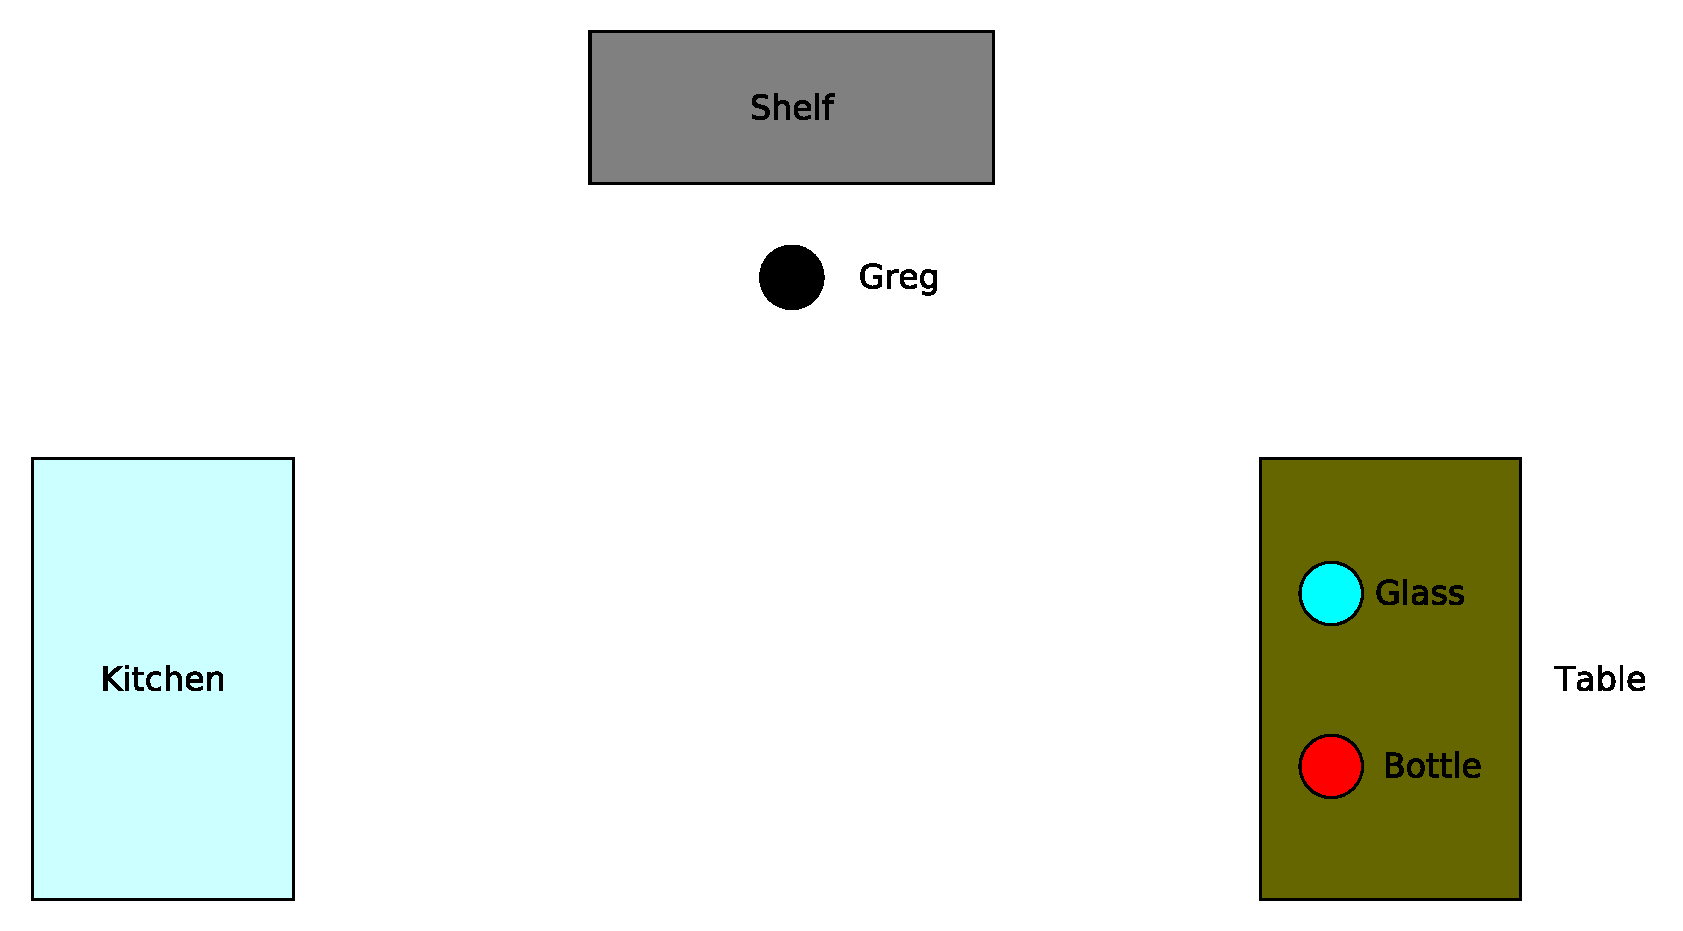
\includegraphics[scale=0.5]{img/situation_assessment/ig_scenario.pdf}
	\caption[IG Example Scenario]{The image shows the set-up for this example scenario. The locations are represented as different rectangles. Greg is represented as a black circle. The glass and bottle are represented, respectively, by a blue circle and a red circle.}
	\label{fig:situation_assessment-ig_scenario}
\end{figure}

We introduce two contexts in the scenario: \textit{HotDay}, representing the fact that the day is particularly warm, and \textit{AlreadyDrank}, representing the fact that the human has recently drank water.

We introduce this possible set of actions in the scenario: taking the bottle, taking the glass, filling the glass using the bottle, drinking from the glass, moving to the kitchen, moving to the table, placing the objects in different locations. We simplify this set to only include the actions relevant to this example, and so we do not include the possibilities for Greg to refill the bottle with water. Also, we consider that Greg can only take a single object at the moment. 

\subsubsection{Building the Intention Graph}

We build a starting IG with the following nodes:
\begin{itemize}
	\item Context Nodes: \textit{HotDay}, \textit{AlreadyDrank}.
	\item Intention Nodes: \textit{DrinkWater}, \textit{ReorderTable}.
	\item Action Nodes: \textit{MoveTable}, \textit{MoveKitchen}. These two actions are introduced in the IG because they are the only ones whose $preconditions$ are currently satisfied, since Greg can move in any location where he is not at the moment.
	\item Observation Nodes: \textit{BodyDistanceTable}, \textit{TowardTable}, \textit{BodyDistanceKitchen}, \textit{TowardKitchen}. The \textit{BodyDistance} nodes represent the distance between Greg and an object, and can assume the values \textit{close}, \textit{medium}, \textit{far}, \textit{out of range}. The \textit{Toward} nodes are \textit{true} if the distance between \textit{Greg} and the object is decreasing, and false otherwise.
\end{itemize}


In this scenario, we precompute the probability table of the causal links between Context Nodes and Intention Nodes, and between Action Nodes and Observaton Nodes. We set a causal link between \textit{HotDay} and \textit{DrinkWater}, and one between \textit{AlreadyDrank} and \textit{ReorderTable}. In both cases, we use the following probability table:

 \begin{table}[h!]
\centering
\begin{tabular}{|c|c|c|}
\hline
Context & \multicolumn{2}{|c|}{Intention} \\ \hline \hline
& 0 & 1 \\ \hline
0  & 0.6 & 0.4 \\ \hline
1 & 0.4 & 0.6 \\ \hline
\end{tabular}
\caption[Belief models in the IG scenario]{Conditioned probabilities of the Intention Nodes in the IG example scenario.}
 \label{table:situation_assessment-ig_intention}    
\end{table}

We consider as slightly more likely that Greg wants to drink water in a Hot Day, and that he wants to reorder the table if he drank recently.

We set a causal link between each action and its observation nodes. For example, \textit{MoveTable} will have a causal link with \textit{BodyDistanceTable} and \textit{TowardTable}. In both actions, we use the following probability tables:

 \begin{table}[h!]
\centering
\begin{tabular}{|c|c|c|}
\hline
Action & \multicolumn{2}{|c|}{Toward} \\ \hline \hline
& 0 & 1 \\ \hline
0  & 0.8 & 0.2 \\ \hline
1 & 0.2 & 0.8 \\  \hline
\end{tabular}
\caption[Belief models in the IG scenario]{Conditioned probabilities of the Toward Nodes in the IG example scenario.}
 \label{table:situation_assessment-ig_toward}    
\end{table}

 \begin{table}[h!]
\centering
\begin{tabular}{|c|c|c|c|c|}
\hline
Action & \multicolumn{4}{|c|}{Distance} \\ \hline \hline
& Close & Medium & Far & Out of Range \\ \hline
0  & 0.16 & 0.2 & 0.25 & 0.39 \\ \hline
1 & 0.39 & 0.25 & 0.2 & 0.16 \\ \hline
\end{tabular}
\caption[Belief models in the IG scenario]{Conditioned probabilities of the Distance Nodes in the IG example scenario.}
 \label{table:situation_assessment-ig_distance}    
\end{table}

If Greg is executing an action, it  more likely that he is moving toward the action's $target$. For example, the \textit{MoveTable} action is more likely the closer Greg is to the table and if the distance to it is decreasing.

\subsubsection{Building the Human MDPs}

To set the conditioned probabilities between Intention and Action Nodes, we created two different MDPs, each related to one of the intentions. We will now show the state space $S$, action set $A$ and reward function $R$  of the two MDPs. We do not include the transition function of the model as it is extensive and does not help understanding this example.

\begin{itemize}
\item DrinkWater:
\begin{itemize}
\item $S$: $\{agent\_isAt, glass\_isAt, bottle\_isAt, bottle\_capacity, glass\_capacity\}$.
\item $A$: $\{agent\_move\_table, agent\_move\_kitchen, agent\_move\_shelf, agent\_take\_bottle, \\ 
agent\_take\_glass, 
agent\_fill\_glass\_bottle, agent\_drink\_glass, agent\_place\_bottle\_table, \\ agent\_place\_bottle\_kitchen, agent\_place\_bottle\_shelf, agent\_place\_glass\_table, \\ agent\_place\_glass\_kitchen, agent\_place\_glass\_shelf\}$.
\item $R(s,a)=1000 \quad \text{if} \\
glass\_isAt==agent\_isAt \; \text{AND} \; glass\_capacity==1  \; \text{AND} \; a==agent\_drink\_glass$.
\end{itemize}


\item ReorderTable:
\begin{itemize}
\item $S$: $\{agent\_isAt, glass\_isAt, bottle\_isAt\}$.
\item $A$: $\{agent\_move\_table, agent\_move\_kitchen, agent\_move\_shelf, agent\_take\_bottle,\\ agent\_take\_glass, 
agent\_place\_glass\_kitchen, agent\_place\_bottle\_kitchen\}$.
\item $R(s,a)=1000 \quad \text{if} \\
(glass\_isAt==kitchen \; \text{AND} \; bottle\_isAt==human \; \text{AND} \; a==human\_place\_bottle\_kitchen)  \\
 \text{OR} \\
 (glass\_isAt==human \; \text{AND} \; bottle\_isAt==kitchen \; \text{AND} \; a==human\_place\_glass\_kitchen)$.
\end{itemize}
\end{itemize}

After solving these MDPs we used their action value functions to compute the conditioned probabilities for the Action Nodes, as shown in \ref{sec:situation_assessment-action_evaluation}.

\subsubsection{Simulated Run}

We will now show a simulated run of this scenario in three steps. This run was created by introducing a stream of observations in the system, including the actions that Greg will perform. We consider that Greg's intention in this example is \textit{Drink Water}. We will conduct three different tests for each step:
\begin{itemize}
	\item Test 1. We create the IG using the human's mental belief state to compute the causal links between action and intention nodes. We do not use context to help disambiguate the intentions.
	\item Test 2. We add contextual information to Test 1, setting \textit{HotDay} to \textit{true} and \textit{RecentlyDrank} to \textit{false}.
	\item Test 3. We do not use contextual information and use the robot's mental belief state to compute the causal links between action and intention nodes. This means that the robot will evaluate Greg's action by considering that he knows that the bottle is currently empty (even though he does not know).
\end{itemize}

We will now describe and discuss these stages:
\begin{itemize}
	\item Greg is approaching the \textit{table}, as shown in figure ~\ref{fig:situation_assessment-ig_exp1}. The observations are updated correspondigly, and the probabilities of the actions are computed. The action \textit{MoveTable} has the highest probability. 
		\begin{itemize}
			\item Test 1. At this stage, the system is not able to infer the correct intention. Greg could be going to the \textit{table} to take the objects and bring them to the \textit{kitchen} or to drink water. The probability of the two intentions is both 0.50.
			\item Test 2. By using context, the system is already able to infer the correct intention. The probability of \textit{DrinkWater} becomes 0.69, and that of \textit{ReorderTable} 0.3. The robot could already fire a proactive behavior to inform Greg that the \textit{bottle} is, in fact, empty.
			\item Test 3. Without context, the system thinks that Greg is trying to reorder the table, since it is not possible to drink water because the \textit{bottle} is empty. The system would infer a wrong intention.
		\end{itemize}
	\item Greg has arrived to the \textit{table}, as shown in figure as shown in figure ~\ref{fig:situation_assessment-ig_exp2}. The $postconditions$ of the action are added to the mental models of the robot and of Greg, changing Greg's location. The system creates a new IG, setting as actions those whose $preconditions$ are now satisfied: \textit{MoveKitchen}, \textit{MoveShelf}, \textit{TakeGlass}, and \textit{TakeBottle}. At this point, Greg's hand moves toward the \textit{bottle}, and the observations nodes are set appropriately.
		\begin{itemize}
			\item Test 1. The system is still not able to disambiguate between the two intentions. Greg could be taking the  \textit{bottle} to fill the \textit{glass} or to bring it to the \textit{kitchen}.
			\item Test 2. In this case, the context is still providing the missing information to understand that Greg wants to drink water.
			\item Test 3. In this case, since it is not possible to drink water in the robot's mental belief, the system is still inferring the wrong intention.
		\end{itemize} 
	\item Greg has taken the \textit{bottle}, and is now moving it to the \textit{glass}, as shown in figure ~\ref{fig:situation_assessment-ig_exp3}. A new IG is created, containing the actions that are now executable: \textit{MoveKitchen}, \textit{MoveShelf}, \textit{PlaceBottleTable}, and \textit{FillGlass}. In test 3, the IG created would not contain the action to fill the glass with water, since it is not executable in the robot's mental belief model, where the \textit{bottle} is empty.
		\begin{itemize}
			\item Test 1. At this point, the system has enough information to understand that Greg's intention is \textit{DrinkWater}, which assumes a probability of 0.90. The system can now fire a proactive behavior, with the robot informing Greg of the divergent belief. Even tought the action \textit{PlaceBottleTable} and \textit{FillGlass} could be ambiguous from a geometric point of view (since in both cases, the arm of the human will approach the table), the system could infer that the action performed was \textit{FillGlass} since it is more \textit{useful} in the current situation and with the considered intentions.
			\item Test 2. Context confirms this intention, bringing the probability to 0.99.
			\item Test 3. In this case, Greg's movement would not be understood, since in the robot's mental belief model it is not possible to fill the glass with water.
		\end{itemize}
\end{itemize}

 \begin{figure}[ht!]
	\centering
	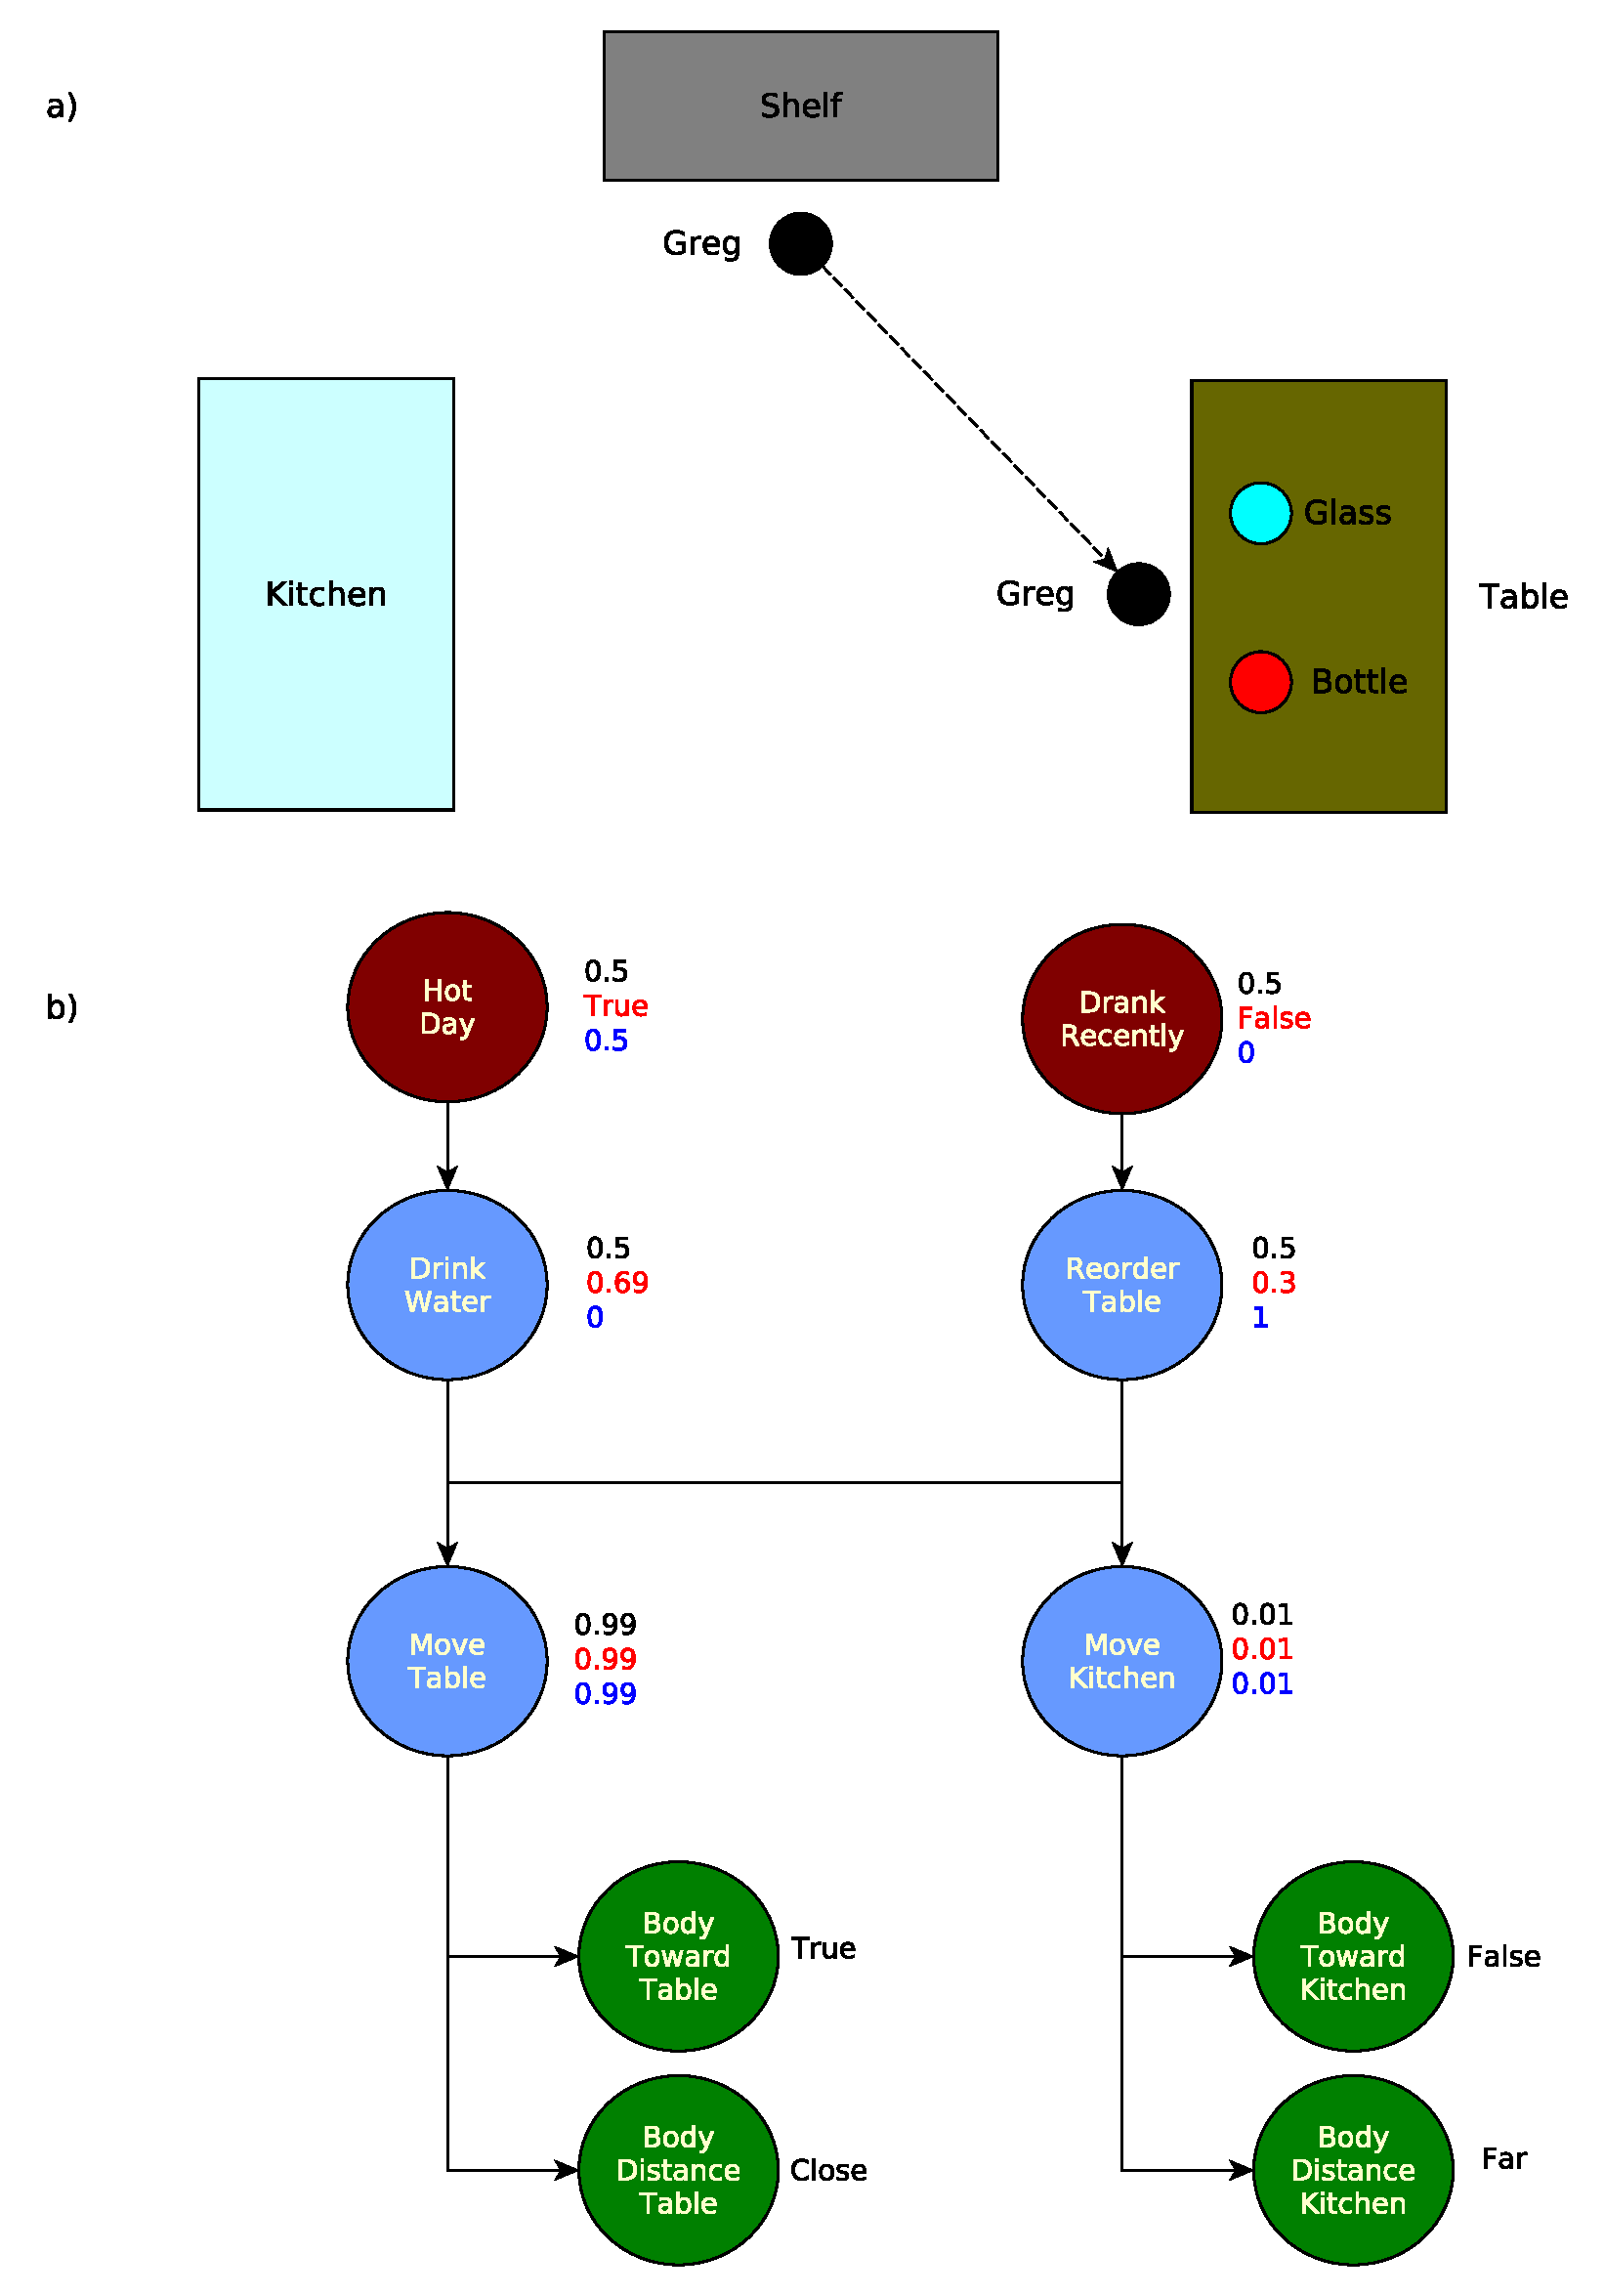
\includegraphics[scale=0.4]{img/situation_assessment/ig_exp1.pdf}
	\caption[IG Example 1]{a) Greg, represented as a black circle, is approaching the table. The two black circles correspond to his starting and ending location, with the dotted arrow showing the direction. b) The corresponding IG graph. Nodes are represented as circles and causal links as arrows. Intention and action nodes as represented as blue. Observation nodes are represented as green to show that we consider them as evidence, fixing their values. Context nodes are represented in yellow to mean that in the first and third test they are treated as standard nodes, and in the second as evidence.
 	 For each node we show the probability that its value is true or its current value, if it is treated as evidence. We show three different values for each node: the black one shows the value if we compute the probability by using the human's mental belief (test 1), the red if we use the human's mental belief and treat context nodes as evidence (test 2), and the blue if we do not use context and use the robot's mental belief for the computation (test 3). Test 1 shows that at this point the system is not able to disambiguate between the two intention, which have a value of 0.50. Test 2 shows that context would help the robot to infer correctly the intention. Test 3 shows that by not using the human's mental belief the robot would discard the drink water intention, considering it not achievable.}
	\label{fig:situation_assessment-ig_exp1}
\end{figure}

\clearpage

\hfill
 \begin{figure}[ht!]
	\centering
	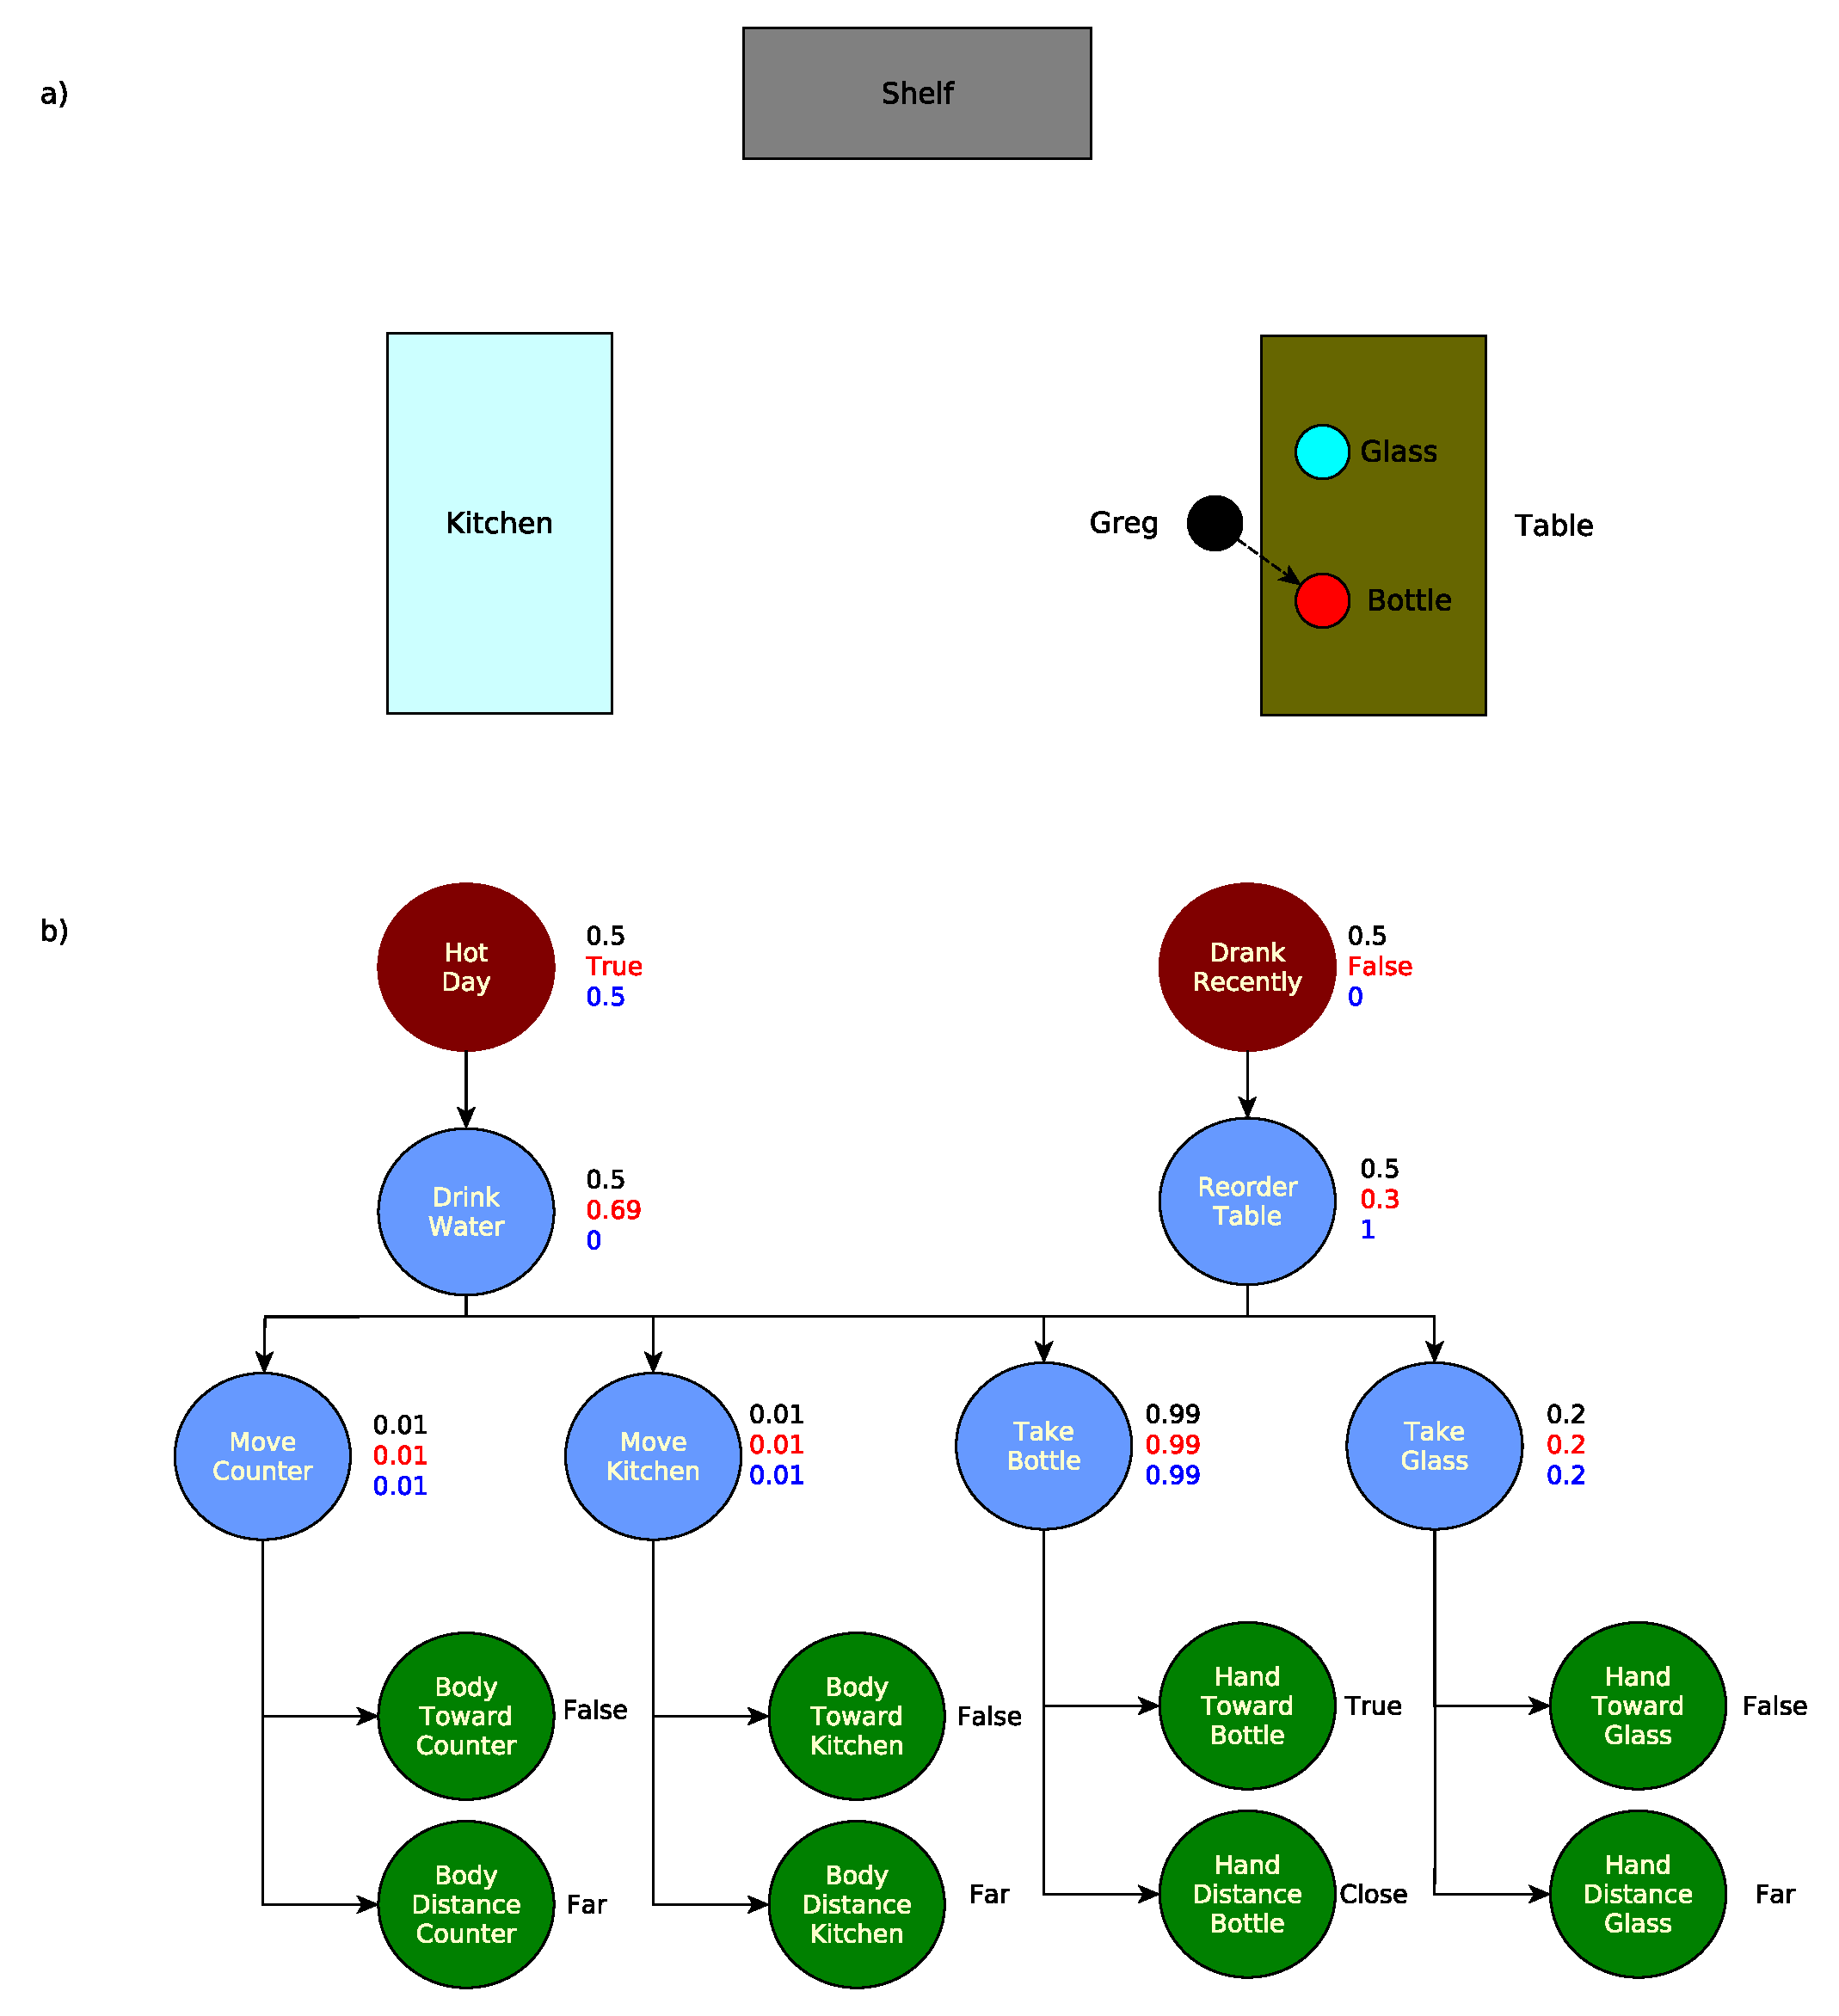
\includegraphics[scale=0.4]{img/situation_assessment/ig_exp2.pdf}
	\caption[IG Example 2]{a) Greg's hand is approaching the bottle. b) The corresponding IG graph. As before, test 1 is shown in black, test 2 in red, and test 3 in blue. The results of 
	the test are very similar to the previous time step, shown in \ref{fig:situation_assessment-ig_exp1}.}
	\label{fig:situation_assessment-ig_exp2}
\end{figure}

\clearpage
 \begin{figure}[ht!]
	\centering
	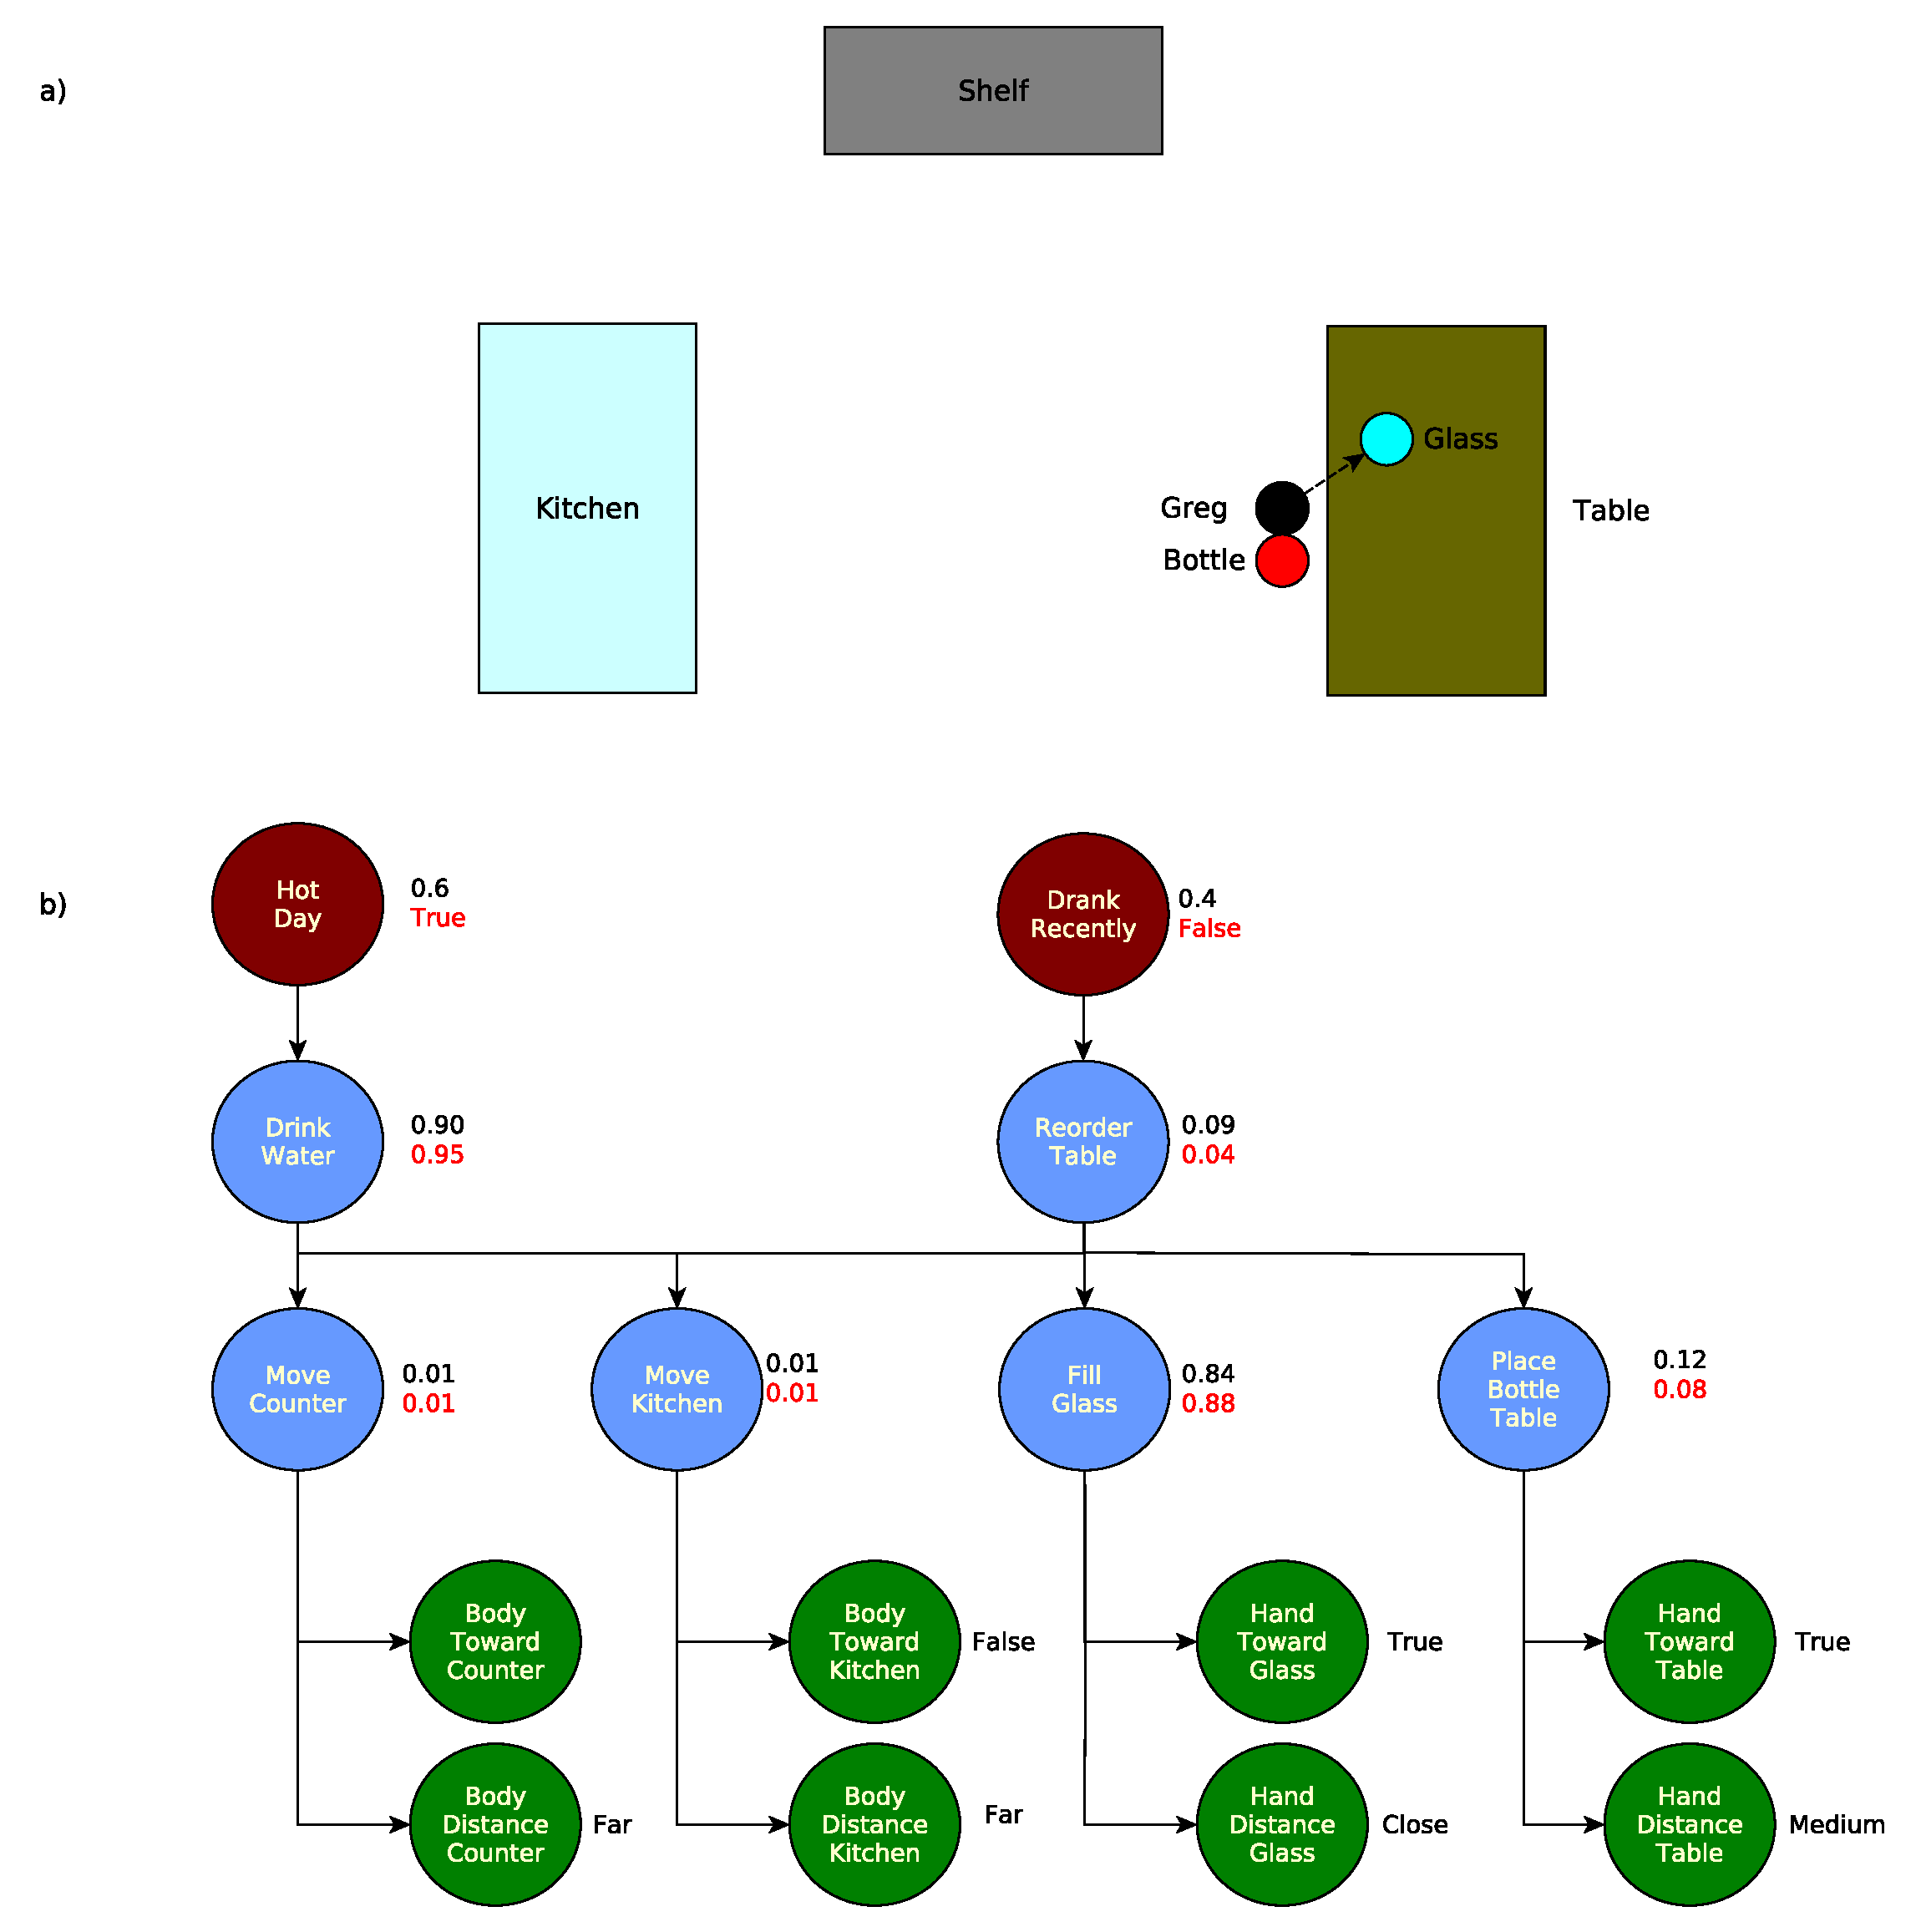
\includegraphics[scale=0.4]{img/situation_assessment/ig_exp3.pdf}
	\caption[IG Example 3]{a) Greg has taken the bottle, shown by placing the red circle and black circles close. His hand, with the bottle, is now approaching the glass b) The corresponding IG graph. As before, test 1 is shown in black and test 2 in red. Test 3 is not shown since the fill glass action would not be executable in the robot's mental belief model, and so the corresponding IG would be different. In test 1 the system has now sufficient information to infer the corrent intention, which has a value of 0.98. Test 2 confirms this choice.}
	\label{fig:situation_assessment-ig_exp3}
\end{figure}
\clearpage

\subsection{Discussion}

This component is able to estimate the likelihood of a human's intention by combining BNs, MDPs, geometrical reasoning, and the capacity to model human's beliefs. Contextual information can further help to disambiguate the inference process. We will show in the next section that the system is able to approach the capacity of humans to infer intentions. 

Another advantage of our approach is its good scalability. Computing the probabilities in a BN can be done using efficient and well know algorithms, which scale well with the size of the network, meaning that the IG is able to accomodate the addition of new actions, observations and contexts. 

Adding a new intention means creating and solving another MDP. Since this process is done offline this would not impact the run of the system. When computing the conditional probabilities of the action nodes, the system uses the action value function of the MDPs, which is stored in memory and can be directly accessed.
.
\section{Experiments and Discussion}
\label{sec:situation_assessment-experiments}
\subsection{Case Study}
Evaluating the capacity of the system to estimate human intentions is not easy, since intentions are not directly observable. A possible solution, as shown in \cite{baker2014modeling}, is comparing the estimation of human intentions, performed by other humans, with the predictions of our system. In order to perform this comparison we created a user study where we showed participants several videos, asking them to estimate the likelihood of a set of intentions  for each video, and collected their results. The same tests where simulated on a robot, streaming as input a sequence of observations  corresponding to the actions shown in the video (e.g. if the video shows a human approaching the table, we will stream to the robot a trajectory of coordinates that leads to the table position). All of the test videos ended in a situation of ambiguity. For example, in one test we showed a human approaching a table with different objects, and stopped the video before users could see which object the human wanted to take. Some videos include more information than others, like comments by humans or situations that help to disambiguate the intention. 

We have performed an equivalence test, comparing users' intentions predictions with those of the robot, following the two one-sided tests (TOST) approach. We choose as a threshold for equivalence the standard deviation $\sigma$ of the users' answers. The idea behind this choice is that, if the robot's answers are closer than a standard deviation to the average human answers, its predictions are comparable to an average human answer from our user group. 

We defined our hypothesis as follow: 
\begin{itemize}
\item $H_0$: $\mu_{hi}-\mu_{ri}\leq-\sigma_{hi}$ \; \text{OR} \; $\mu_{hi}-\mu_{ri}\geq\sigma_{hi}$ 
\item $H_A$: $-\sigma_{hi}<\mu_{hi}-\mu_{ri}<\sigma_{hi}$  
\end{itemize}
where $\mu_{hi}$ and $\mu_{ri}$ are the human average and the robot's answer for test $i$, $\sigma_{hi}$ is the variance of the human answers for test $i$.

We have performed tests to evaluate: a) prediction in absence of clues, b) prediction in the presence of contextual clues, c) prediction in the presence of belief state clues.

We built a household environment with a fixed set of furniture: a \textit{Kitchen Shelf}, a \textit{Table}, a \textit{Sofa}, and a \textit{Chair}. In this environment, we created two scenarios, composed by several tests, with two agents, \textit{Max} and \textit{Bob}, performing different actions. Each scenario contained a set of objects, and a constrained set of intentions. For the tests related to belief states, we start by showing the users a specific sequence of events, allowing them to build a mental model of the agents. A corresponding simulated sequence will be streamed to the robot for this test.
We will describe in details the two scenarios and the relative tests.

\subsubsection{Cookie Scenario}
\begin{itemize}
\item Objects: a \textit{Cookie Box}, a \textit{Mug}, and a \textit{Bottle of Water} were placed on the \textit{Table}, close to each other. A pack of \textit{Cookies} was placed on the \textit{Kitchen Shelf}. The \textit{Cookie Box} could contain, or not, \textit{Cookies}.
\item Intentions: \textit{Eating a Cookie}, \textit{Drinking Water}, \textit{Reading the Book}.
\item Tests:
\begin{itemize}
	\item \textit{No Clues}: \textit{Max} approaches the \textit{Table}.
    \item \textit{Contextual Clues}: \textit{Max} approaches the \textit{Table} commenting on the warmth of the day.
	\item \textit{Divergent Belief Max}: \textit{Max} approaches the \textit{Table}.
	\item \textit{Divergent Belief Bob}: \textit{Bob} approaches the \textit{Table}.
\end{itemize}
\item  \textit{Divergent Belief Event}:  \textit{Max} and \textit{Bob} are chatting on the \textit{Sofa}. Max eats the last \textit{Cookie} from the \textit{Cookie Box} before closing it and leaving. While \textit{Max} is away, \textit{Bob} takes \textit{Cookies} from the \textit{Kitchen Shelf}, fills the \textit{Cookie Box} with them, and closes it, before leaving.
\end{itemize}

The \textit{Divergent Belief Event} was shown to the users (and its simulation streamed to the robot) between the \textit{Contextual Clues} and the \textit{Divergent Belief Max} events. 


We deliberately included an intention, \textit{Reading the Book}, without placing a book in the visible environment, introducing a confusing element in the scenario. This scenario can be seen in figure~\ref{fig:situation_assessment-cookie}.


 \begin{figure}[ht!]
	\centering
	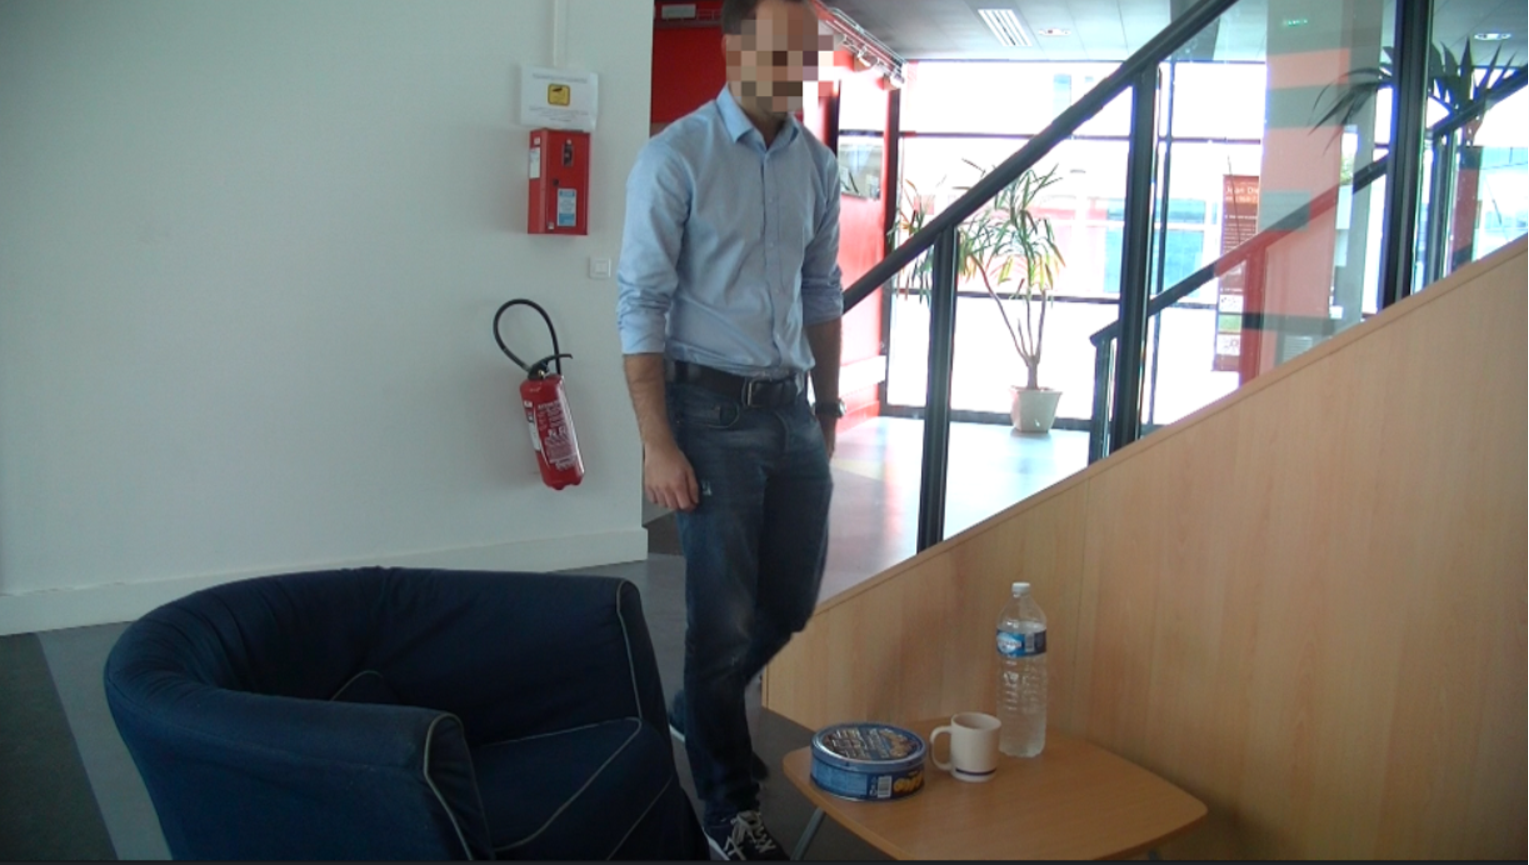
\includegraphics[scale=0.5]{img/situation_assessment/cookie1-blur.pdf}
	\caption{The cookie intention scenario}
	\label{fig:situation_assessment-cookie}
\end{figure}


\subsubsection{Keys Scenario}
\begin{itemize}
\item Objects: A \textit{Box} was placed on the \textit{Table}, that partially occluded the sight of people approaching. A \textit{Book} and a \textit{Mug} where placed behind the \textit{Box}, so that they could be seen from the sofa but not from approaching people.
\item Intentions: \textit{Taking the Mug}, \textit{Taking the Keys}, \textit{Reading the Book}.
\item Tests and Events:
\begin{itemize}
\item \textit{No Clues}: \textit{Max} approaches the \textit{Table}.
\item\textit{Contextual Clues}: \textit{Max} approaches the \textit{Table} in a hurry, while putting on a coat.
\item \textit{Divergent Belief Max}: \textit{Max} approaches the \textit{Table} in a hurry, while putting on a coat.
\end{itemize}
\item \textit{Divergent Belief Event}: \textit{Max} is sitting on the \textit{Table}, drinking from the \textit{Mug}, while having the \textit{Keys} in his hands. His phone rings, so he drops the \textit{Keys} and the \textit{Mug} on the \textit{Table}, behind the \textit{Box}, and leaves the room. While \textit{Max} is away, \textit{Bob} comes and sits on the \textit{Sofa}, reading a \textit{Book}. When he sees the \textit{Keys}, he takes them, places the \textit{Book} on the \textit{Table}, and leaves.
\end{itemize}

The \textit{Divergent Belief Event} was shown to the users (and its simulation streamed to the robot) between \textit{Contextual Clues} and the \textit{Divegent Belief Max} events. This scenario can be seen in figure~\ref{fig:situation_assessment-keys}

 \begin{figure}[ht!]
	\centering
	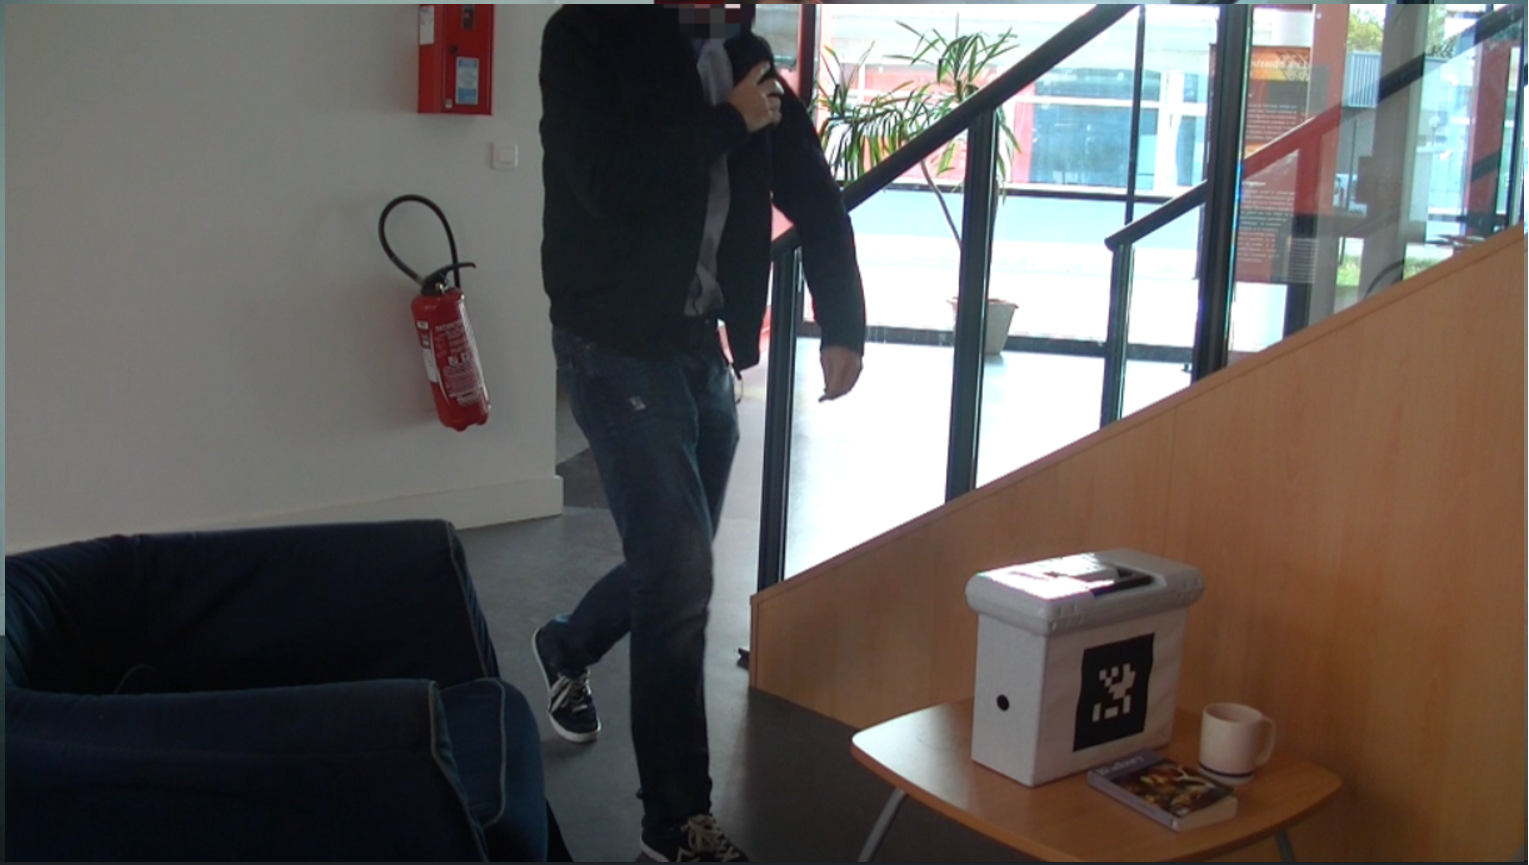
\includegraphics[scale=0.5]{img/situation_assessment/keys2-blur.pdf}
	\caption{The keys intention scenario}
	\label{fig:situation_assessment-keys}
\end{figure}

\subsection{User Study}
We built an online user study, where we presented videos related to the tests and events of the two scenarios to users, who had to evaluate the likelihood of each intentions of the scenario
on a five-level Likert scale. The user study was conducted in three languages, with users living in two different countries\footnote{A version of this user study was provided at http://goo.gl/forms/YiuFHnF63c}. We collected answers from 78 adults, performed an average, and converted them to percentile scores, in order to compare them with the robot's predictions.

Looking at users' answers (figure \ref{fig:situation_assessment-user_study_results}), we can see that, in the absence of clues, people rated similarly the two intentions related to visible objects. Contextual clues had the highest influence on users' ratings. This is particularly visible in the \textit{Contextual Clues} test of the \textit{Keys Scenario}, where users chose as the most likely intention \textit{Take Keys}, even if no keys were visible in the video. Divergent beliefs also influenced users decisions, but not as strongly as context. The strongest responses, over all, where given by the \textit{Divergent Belief Max} test on \textit{Keys Scenario}, which uses both divergent belief and contextual information.

\subsection{Robot implementation}
At the start of a scenario the robot scanned the environment, building a model of its world state. With our perception capacities, we can not detect if the cookie box is full or empty, and so we consider it as full at the start of a test, and update its value using the $postconditions$ of inferred human actions. We consider the box as empty when we infer that a human has taken a cookie from inside, and as full when we infer that a human has put a cookie in it.

We have built different IGs for the scenarios. Each test had a different graph, related to its main agent. We considered three different Context Nodes for these IGs: $Hot Day$, true when the day is particularly warm; $Break Time$, true when the agents are taking a pause; $Time to Leave$, true when it's late in the day, and the humans usually leave work and return home.

As previously said, we chose to follow \cite{Liu2014} in order to learn the link between Contexts and Intentions. We created a second user study with 15 users, in which we presented a set of 5 scenarios, each one related to one of the intentions of our tests. For each scenario we asked the users to rate the perceived link, on a five-level Likert scale, between the intention and our three contexts. We averaged users' answers and calculated the conditional probabilities between context nodes and intention nodes from these averages.


In the \textit{Cookie Scenario} the graph for the tests is constructed from the following nodes:
\begin{itemize}
\item Context Nodes: \textit{Hot Day}, \textit{Break Time}, \textit{Time to Leave}
\item Intention Nodes: \textit{Fill Cookie Box}, \textit{Eat Cookie}, \textit{Drink Water}, \textit{Read Book}.
\item Action Nodes: \textit{Move to Table}, \textit{Move to Kitchen}.
\item Observation Nodes: distance of the agent body and hand to each action's associated \textit{target}.
\end{itemize}

We introduce the \textit{Fill Cookie Box} intention, not present in the human test, to allow the robot to detect when Bob fills the \textit{Cookie Box} during the \textit{Divergent Belief Event}.

Our robot does not have speech recognition capacities. We simulated this capacities, and set Context Nodes to plausible values, that could be extracted by watching the videos. For the \textit{Contextual Clues} test, we set the value of \textit{Hot Day} to true (since Max is commenting about the temperature), and \textit{Break Time}, and \textit{Time to Leave} to false (since no data in the video points to one of these contexts being true. Max and Bob seem to have taken a break from work before the other events are shown, in the Divergent Belief Event).
%Our robot doesn't have speech recognition capacities. and for \textit{Contextual Clues} test, set the value of \textit{Hot Day} to \textit{true}, and the value of \textit{Break Time} to \textit{false}, i.e. the robot knows that it is not the usual time for the agents to take a break.

\textit{Divergent Belief Event}, \textit{Divergent Belief Max}, and \textit{Divergent Belief Bob} were showed sequentially to the robot, which updated the agents' mental models and created new IGs accordingly. During the \textit{Divergent Belief Event} several IGs need to be created with different action and observation nodes, to follow the sequence of actions by the two agents. For example, when \textit{Max} leaves the room, \textit{Bob} has the possibility to execute the actions \textit{Take Mug}, \textit{Take Water Bottle}, \textit{Open Cookie Box}, \textit{Move to Kitchen Shelf} or \textit{Leave Room}. Intention and Context nodes remains the same in all the IGs of the scenario.


The \textit{Keys Scenario} has a similar IG, with the following differences.
\begin{itemize}
\item Context Nodes: \textit{Hot Day}, \textit{Break Time} and \textit{Time to Leave}.
\item Intention Nodes: \textit{Drink Water}, \textit{Take Keys}, \textit{Read Book}.
\end{itemize}

Action Nodes and Observation Nodes are the same as the previous scenario, and follow the same ideas during the \textit{Divergent Belief Event}. An example of IG used in the tests can be seen in figure \ref{fig:situation_assessment-intention_graph}. For the \textit{Contextual Clues} and \textit{Divergent Belief} test, we set the \textit{Time to Leave} context value to \textit{true} (since Max is putting a coat and seems in a hurry), and other context node values to \textit{false}. Using the component described in the previous sections, and these IGs the robot was able to obtain predictions from the user actions.

\subsection{Discussion}
\label{sec:discussion}
We performed TOST tests for each intention in the scenarios, comparing the humans' answers with the robot's, for a total of 21 tests. We calculated p-values and performed our tests using a significance value $\alpha=0.05$.

Analyzing the results of our equivalence tests, shown in figure \ref{fig:situation_assessment-user_study_results}, produces some interesting information.
\begin{itemize}
\item The behavior of our system is often close to human capacities. 19 tests out of 21 passed our requirements for significance level, often with very low p-value scores. 
\item Context and Divergent Belief are necessary. A system without these skills would only have been able to model properly the \textit{No Clues} cases. 
\item There are still some missing aspects in our system. We failed to reject the null hypothesis for two tests. In \textit{Divergent Belief Bob} users rated higher the \textit{Eat Cookie} intention than the \textit{Drink Water} intention, possibly because they thought that since \textit{Bob} filled the \textit{Cookie Box} he may want to eat a \textit{Cookie}. This makes us think that humans use deep temporal reasoning to evaluate intentions, considering the whole history of actions performed by agents.  
\end{itemize}
 \begin{figure}[ht!]
	\centering
	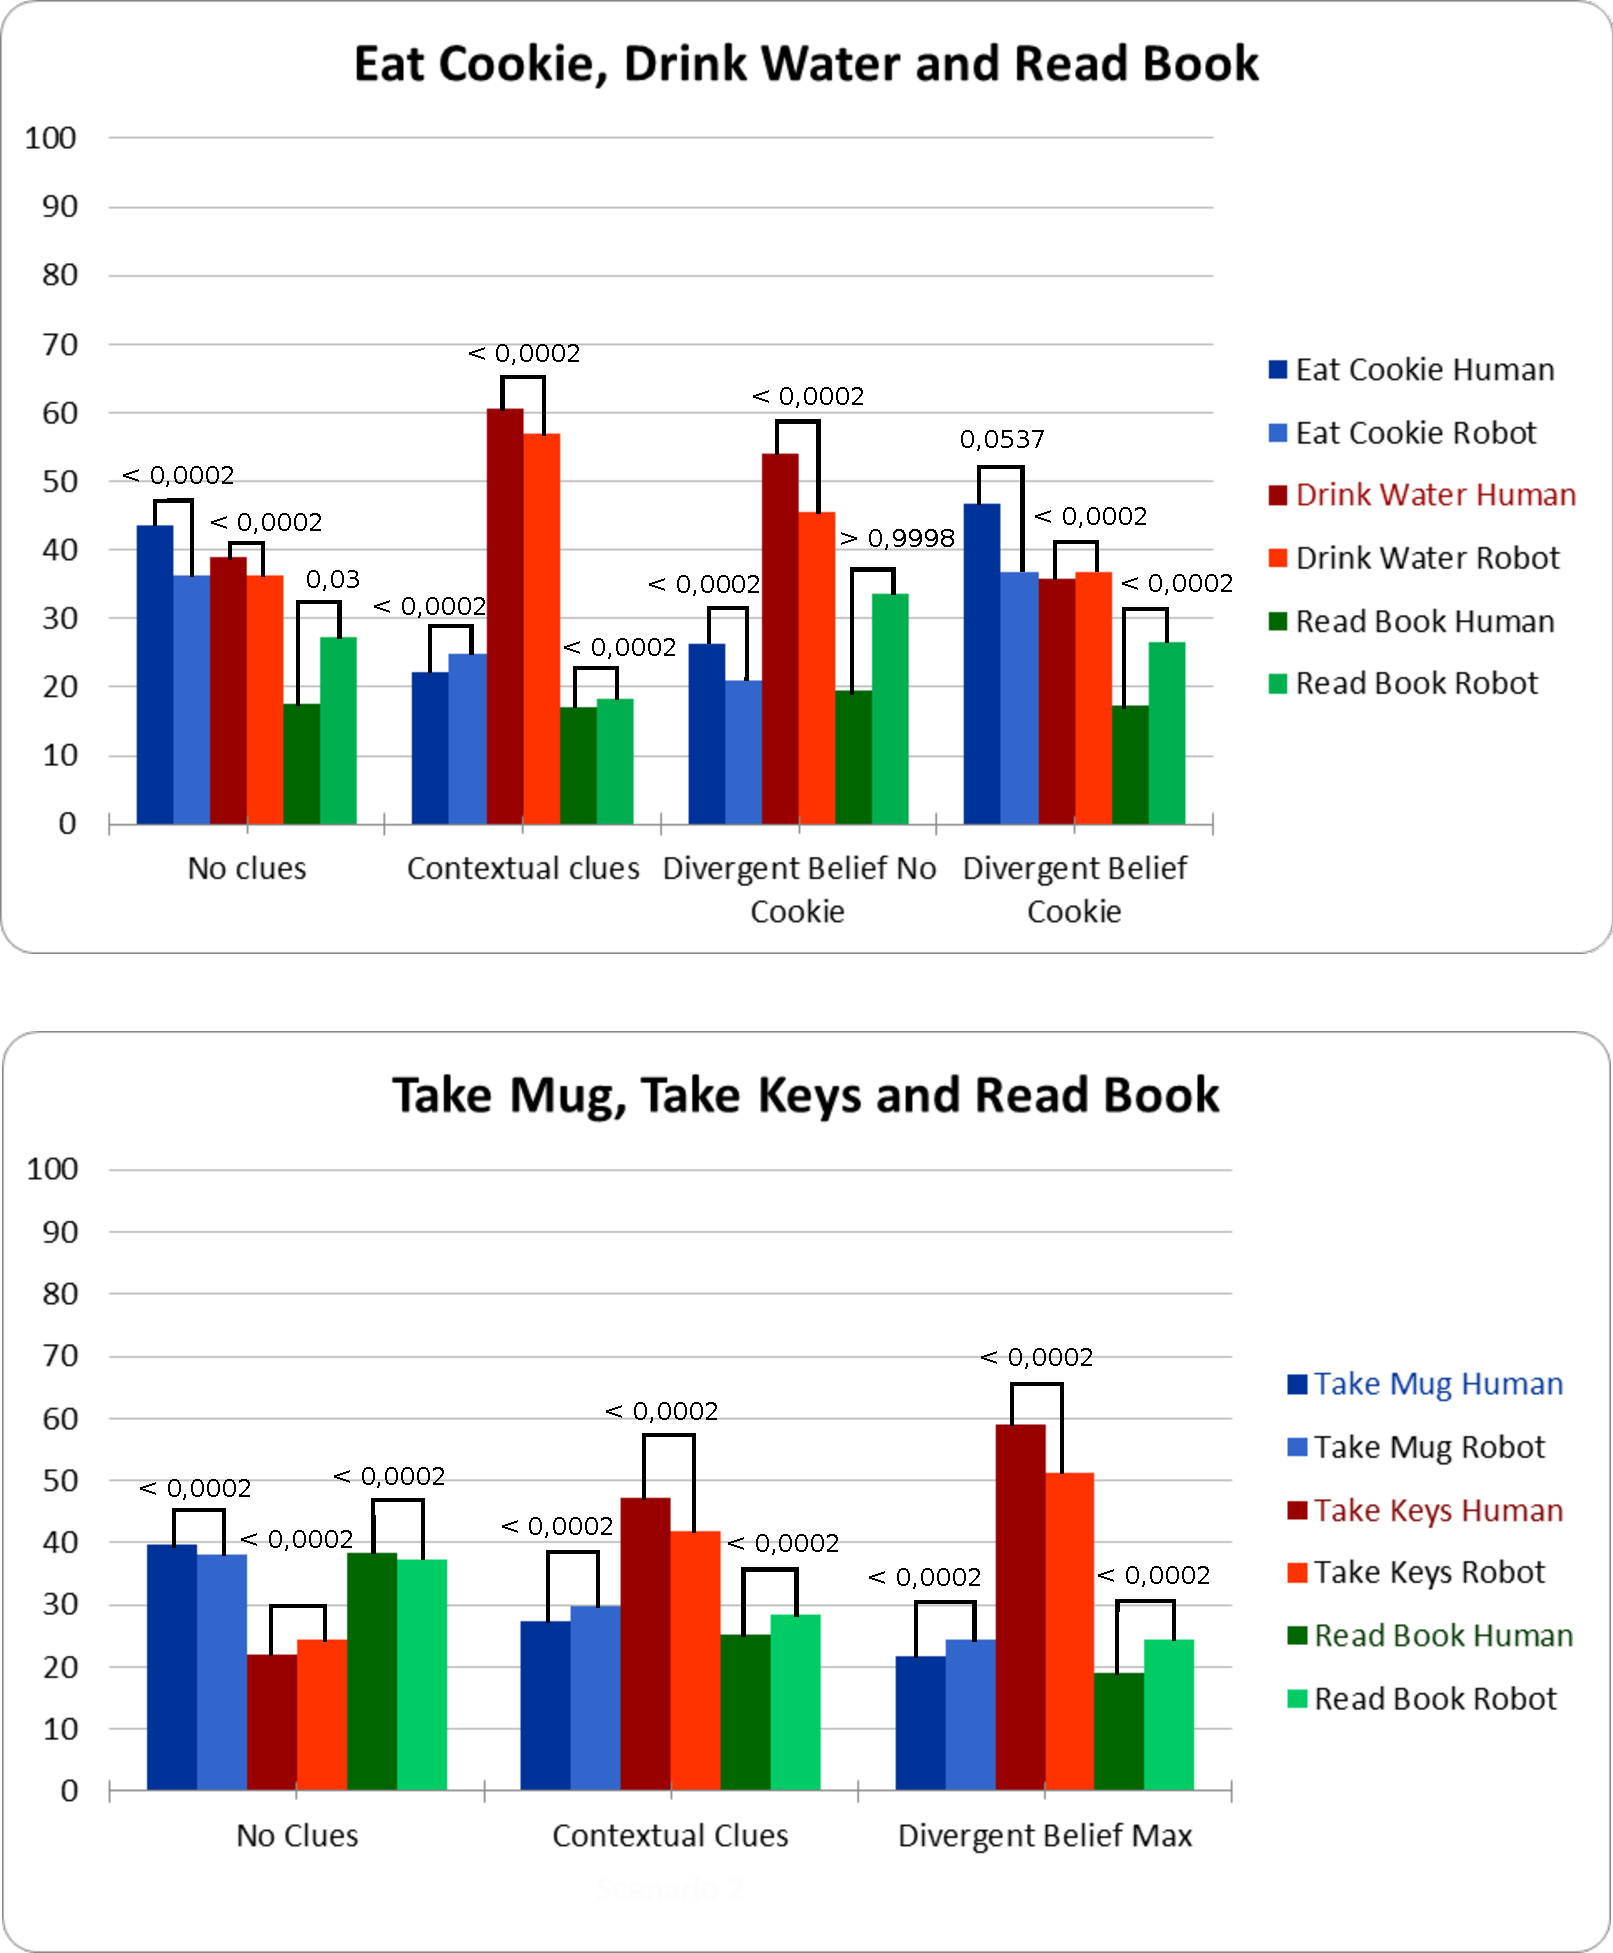
\includegraphics[clip,scale=0.5]{img/situation_assessment/pvalues1.pdf}
	\caption[Experiment results]{Experiment results. Results from the two scenarios are represented as graphs. Intentions, as estimated by the humans and the robot, are represented by different colors, as shown in the legend of the graphs, with estimations of the same intention by the robot or the human placed in adjacent position. Each column represents the likelihood of an intention, expressed as a percentile score. P-values from the equivalence tests are shown, linking the estimation of an intention by the humans and by the robot.}
	\label{fig:situation_assessment-user_study_results}
\end{figure}



 
